% COS30049 Assignment 2 -- delivery plan (not the report).
% Group HCMC_COS30049.1_4. Compile with pdfLaTeX twice: pdflatex main && pdflatex main
\documentclass[a4paper,11pt]{article}

% ---------------------------------------------------------------- page and fonts
\usepackage[margin=2.3cm]{geometry}
\usepackage[T1]{fontenc}
\usepackage[utf8]{inputenc}
\usepackage{lmodern}
\usepackage{microtype}
\usepackage{parskip}
\setlength{\emergencystretch}{2em} % lets lines with long monospace commands break cleanly
\DeclareUnicodeCharacter{2192}{\ensuremath{\rightarrow}}
\DeclareUnicodeCharacter{2265}{\ensuremath{\geq}}
\DeclareUnicodeCharacter{2264}{\ensuremath{\leq}}
\DeclareUnicodeCharacter{00D7}{\ensuremath{\times}}
\DeclareUnicodeCharacter{2212}{\ensuremath{-}}
\DeclareUnicodeCharacter{2248}{\ensuremath{\approx}}

% ---------------------------------------------------------------- tables
\usepackage{array}
\usepackage{booktabs}
\usepackage{tabularx}
\usepackage{longtable}
\usepackage{multirow}
\usepackage{colortbl}
\renewcommand{\arraystretch}{1.22}
\newcolumntype{L}[1]{>{\raggedright\arraybackslash\hspace{0pt}}p{#1}}
\newcolumntype{Y}{>{\raggedright\arraybackslash\hspace{0pt}}X}
\newcolumntype{C}[1]{>{\centering\arraybackslash}p{#1}}

% ---------------------------------------------------------------- figures and drawing
\usepackage{graphicx}
\usepackage{float}
\usepackage{caption}
\captionsetup{font=small, labelfont=bf}
\captionsetup[table]{position=top}
\usepackage{tikz}
\usetikzlibrary{arrows.meta, positioning, calc, fit, backgrounds, shapes.geometric}

% ---------------------------------------------------------------- text
\usepackage{amsmath}
\usepackage{amssymb}
\usepackage{enumitem}
\setlist{itemsep=2pt, topsep=3pt, parsep=0pt}
\usepackage{xcolor}
\usepackage{pifont}
\usepackage{titlesec}
\usepackage{fancyhdr}
\usepackage{url}
\usepackage{listings}
\usepackage[skins,breakable]{tcolorbox}

\definecolor{ink}{HTML}{1F2933}
\definecolor{accent}{HTML}{1D4ED8}
\definecolor{accentsoft}{HTML}{E8EEFC}
\definecolor{okgreen}{HTML}{15803D}
\definecolor{oksoft}{HTML}{E7F5EC}
\definecolor{warn}{HTML}{B45309}
\definecolor{warnsoft}{HTML}{FDF1E3}
\definecolor{grey}{HTML}{6B7280}
\definecolor{greysoft}{HTML}{F3F4F6}
\definecolor{violet}{HTML}{6D28D9}
\definecolor{violetsoft}{HTML}{F1EBFD}
\definecolor{teal}{HTML}{0F766E}
\definecolor{tealsoft}{HTML}{E6F4F2}

\titleformat{\section}{\Large\bfseries\color{ink}}{\thesection}{0.8em}{}
\titleformat{\subsection}{\large\bfseries\color{ink}}{\thesubsection}{0.7em}{}
\titleformat{\subsubsection}{\normalsize\bfseries\color{ink}}{\thesubsubsection}{0.6em}{}
\titlespacing*{\section}{0pt}{1.4em}{0.6em}
\titlespacing*{\subsection}{0pt}{1.1em}{0.4em}

\pagestyle{fancy}
\fancyhf{}
\fancyhead[L]{\small\color{grey}COS30049 A2 delivery plan}
\fancyhead[R]{\small\color{grey}HCMC\_COS30049.1\_4}
\fancyfoot[C]{\small\thepage}
\renewcommand{\headrulewidth}{0.3pt}

% Boxes. Each one has a single job, so a reader can skim by colour.
\newtcolorbox{decision}[1]{enhanced, breakable, colback=accentsoft, colframe=accent,
  boxrule=0.6pt, arc=2pt, left=6pt, right=6pt, top=4pt, bottom=4pt,
  title={\textbf{Decision:} #1}, fonttitle=\small, coltitle=white}
\newtcolorbox{done}{enhanced, breakable, colback=oksoft, colframe=okgreen,
  boxrule=0.6pt, arc=2pt, left=6pt, right=6pt, top=3pt, bottom=3pt,
  title={\textbf{Done when}}, fonttitle=\small, coltitle=white}
\newtcolorbox{feeds}{enhanced, breakable, colback=violetsoft, colframe=violet,
  boxrule=0.6pt, arc=2pt, left=6pt, right=6pt, top=3pt, bottom=3pt,
  title={\textbf{Feeds the report and rubric}}, fonttitle=\small, coltitle=white}
\newtcolorbox{caution}{enhanced, breakable, colback=warnsoft, colframe=warn,
  boxrule=0.6pt, arc=2pt, left=6pt, right=6pt, top=3pt, bottom=3pt,
  title={\textbf{Watch out}}, fonttitle=\small, coltitle=white}
\newtcolorbox{team}{enhanced, breakable, colback=tealsoft, colframe=teal,
  boxrule=0.6pt, arc=2pt, left=6pt, right=6pt, top=3pt, bottom=3pt,
  title={\textbf{Needs a teammate}}, fonttitle=\small, coltitle=white}
\newtcolorbox{summarybox}{enhanced, breakable, colback=greysoft, colframe=ink,
  boxrule=0.6pt, arc=2pt, left=8pt, right=8pt, top=6pt, bottom=6pt,
  before upper={\setlength{\parskip}{0.5em}}}

% Command blocks. Plain monospace; no shell-escape needed.
\lstdefinestyle{cmd}{basicstyle=\ttfamily\small, backgroundcolor=\color{greysoft},
  frame=single, framerule=0pt, xleftmargin=4pt, xrightmargin=4pt, aboveskip=6pt,
  belowskip=6pt, columns=fullflexible, keepspaces=true, breaklines=true,
  showstringspaces=false, upquote=true}
\lstdefinestyle{py}{style=cmd, language=Python, keywordstyle=\color{accent}\bfseries,
  commentstyle=\color{grey}\itshape, stringstyle=\color{okgreen}}
\lstset{style=cmd}

\newcommand{\code}[1]{\texttt{\detokenize{#1}}}
\newcommand{\fp}[1]{\path{#1}} % file paths, breakable at / and .
\newcommand{\yes}{\textcolor{okgreen}{\ding{51}}}
\newcommand{\no}{\textcolor{warn}{\ding{55}}}
\newcommand{\est}{\textsuperscript{\textcolor{grey}{est.}}}

% Numbered reference list [1]-[N], alphabetical, hanging indent (A1's style).
\newcounter{refnum}
\newenvironment{references}{%
  \sloppy\small\raggedright\begin{list}{[\arabic{refnum}]}{\usecounter{refnum}\setlength{\labelwidth}{2.2em}%
    \setlength{\leftmargin}{2.8em}\setlength{\labelsep}{0.6em}%
    \setlength{\itemsep}{0.45\baselineskip}\setlength{\parsep}{0pt}}}%
  {\end{list}}

\usepackage[hidelinks]{hyperref}
\hypersetup{colorlinks=true, linkcolor=accent, urlcolor=accent, citecolor=accent}

\begin{document}

% ---------------------------------------------------------------- title page
\begin{titlepage}
\thispagestyle{empty}
\vspace*{1.5cm}
{\color{grey}\large COS30049 Computing Technology Innovation Project}\par
\vspace{0.4cm}
{\color{ink}\Huge\bfseries Assignment 2 delivery plan}\par
\vspace{0.3cm}
{\color{ink}\Large Everything that will be built, measured, written and packaged\\ between 20 October and 8 November 2026}\par
\vspace{1.2cm}
\begin{tabularx}{\textwidth}{@{}L{4.2cm}Y@{}}
\toprule
Project & Bitcoin Address Activity Explorer (unusual-activity indicator, never a fraud verdict) \\
Group & HCMC\_COS30049.1\_4 \\
Members & Cam Dan Bui (105967074); Cao Tri Tran (106214726); Le Quang Anh Hoang (106218605); Minh Khang Nguyen (106216803) \\
Plan prepared & Tuesday 20 October 2026 (teaching Week 6, day 36 of the 84-day unit) \\
Assignment 2 due & Sunday 8 November 2026, 23:59 GMT+7 (day 55); 19 days from this plan \\
Planned submission & Saturday 7 November 2026, one day early \\
Training machine & Intel Core i5-12600K, NVIDIA RTX 3060 12 GB, 16 GB DDR4-3600, Windows \\
\bottomrule
\end{tabularx}

\vspace{1cm}
\begin{summarybox}
\textbf{What this document is.} A working plan for finishing every marked part of Assignment 2: the
datasets, the code, the trained models (including two language models trained from scratch on the
machine above), the README and the 3,000-word report. It says what will be done, in what order, with
which commands, how long each step should take, how each step is checked, and which rubric line it
earns.

\textbf{What it is not.} It is not the report and is not submitted. Numbers marked \est{} are
planning estimates that a measured run replaces. Nothing in here is a result.

\textbf{Out of scope here.} The weekly meeting minutes and the contribution form are also submitted
with Assignment 2. The team will handle them separately; Section~\ref{sec:checklist} only lists
them so they are not forgotten.
\end{summarybox}
\vfill
{\small\color{grey}Source documents read for this plan: Week 1--8 lecture slides, seminars and
workshop notebooks; the submitted Assignment 1 report, minutes and contribution form; the
Assignment 1 working files (handover audit, risk register, fix log); the Assignment 2 brief and
rubric; the prototype repository (commit 8375cf0); and the existing \texttt{asm2/} language-model code.}
\end{titlepage}

\tableofcontents
\clearpage

\section{The plan on one page}
\label{sec:summary}

\textbf{Goal.} A full-marks attempt at all 40 points: 12 for the report, 20 for the code and zip
file, and 8 HD points. Every task in this plan is tied to one of those points. If a task earns no
point and nothing else depends on it, it was left out.

\textbf{The marks, checked against the brief.} The breakdown used to start this plan missed one
report line. The report is worth 12 points over \emph{six} criteria, not five:

\begin{center}
\small
\begin{tabularx}{\textwidth}{@{}Y C{1.1cm} Y C{1.1cm}@{}}
\toprule
\textbf{Report} (PDF, up to 3,000 words) & \textbf{Pts} & \textbf{Code and zip file} & \textbf{Pts} \\
\midrule
1. Data collection and processing & 5 & 1. Core functionality & 10 \\
2. Data analysis & 2 & 2. Datasets & 4 \\
3. Justification of model selection & 2 & 3. README (conda set-up, training, prediction) & 2 \\
4. Writing quality and logical structure & 1 & 4. Comments & 2 \\
5. Harvard referencing & 1 & 5. Code structure & 2 \\
\textbf{6. Completeness (every required section)} & \textbf{1} & & \\
\midrule
\textit{Report total} & \textit{12} & \textit{Code total} & \textit{20} \\
\midrule
\multicolumn{2}{@{}l}{\textbf{HD}: additional datasets} & 4 & \\
\multicolumn{2}{@{}l}{\textbf{HD}: additional ML implementations} & 4 & \\
\bottomrule
\end{tabularx}
\end{center}

\textbf{What will be built.}
\begin{enumerate}
  \item \textbf{Our own Bitcoin data.} A frozen snapshot of 25 addresses plus 3 short-history ones
    from the Esplora API, as Assignment 1 promised (DS1). A second, much larger crawl of about
    5,000 address histories (DS2) feeds the transaction language model.
  \item \textbf{Two public labelled datasets.} Elliptic (DS3) and BitcoinHeist (DS4) carry labels
    from their authors, so the brief's accuracy, precision, recall and F1 can be reported honestly.
  \item \textbf{All three model types the brief names.} Clustering (K-Means, DBSCAN) and regression
    (Ridge, random forest, gradient boosting) run on our own data. Classification (logistic
    regression, KNN, random forest, gradient boosting) runs on the labelled datasets. The brief
    needs two types; doing all three removes any doubt.
  \item \textbf{The Assignment 1 methods, kept as extra experiments.} The robust-z baseline,
    Isolation Forest and Local Outlier Factor are still built and evaluated with the label-free
    plan. They are also tested against the Elliptic labels, which shows how often ``unusual''
    and ``labelled illicit'' coincide.
  \item \textbf{Two language models trained from scratch on the RTX 3060.} The first, TxGPT, is a
    small GPT that reads an address's history as a sequence of transaction tokens. It scores how
    surprising each new transaction is, and it is the main HD model. The second is a 152M-parameter
    text model, pretrained on 2B tokens of web text and then taught to chat and to explain flags.
    It becomes the Explorer Assistant, which Assignment 3 can use.
  \item \textbf{A prediction interface.} \code{predict.py} plus a command-line tool, so every model
    can score new input. The README shows how, and the Assignment 3 FastAPI back end can call
    the same functions.
\end{enumerate}

\textbf{How this keeps the Assignment 1 promise.} Assignment 1 ruled out claiming fraud accuracy on
data with no labels (risk 13). That rule still holds. Precision and recall are reported only in two
places. One is datasets whose authors supplied labels. The other is transactions we planted
ourselves, where the true answer is known by construction. The Explorer's wording never changes:
\emph{``Unusual activity requires investigation; it does not indicate wrongdoing.''}

\textbf{The dates that matter.}
\begin{center}
\small
\begin{tabularx}{\textwidth}{@{}L{3.1cm}Y@{}}
\toprule
\textbf{Date} & \textbf{Milestone} \\
\midrule
Wed 21 Oct & Change request CR-06 sent to the team and the tutor. Snapshot DS1 fetched. Text pretraining started on the GPU. \\
Sun 25 Oct & M1: baseline, Isolation Forest and LOF score every snapshot transaction. This is Assignment 1 Objective 2, due 26 Oct. \\
Thu 29 Oct & M2: every model trained and evaluated; results frozen (version 1). \\
Sat 31 Oct & M3: code feature-complete; notebooks re-run from clean. \\
Wed 4 Nov & M4: a teammate rebuilds everything from the README on a clean machine; code frozen. \\
Sat 7 Nov & M5: everything submitted on Canvas. Sunday 8 Nov is spare. \\
\bottomrule
\end{tabularx}
\end{center}

\textbf{The critical path.} DS1 fetch → features → time split and baseline → models → evaluation
→ method selection → report evaluation section → submission. Both language models run on a
parallel GPU lane with about three days of slack. If the text model's pretraining runs long, a
decision gate cuts its token budget (Section~\ref{sec:gate}). It never delays the critical path.

\section{What is submitted and how it is marked}
\label{sec:deliverables}

\subsection{The files that go to Canvas}

One member submits everything on behalf of the group. The brief wants files named after the group,
so this plan keeps the Assignment 1 pattern.

\begin{center}
\small
\begin{tabularx}{\textwidth}{@{}L{6.4cm}Y@{}}
\toprule
\textbf{File} & \textbf{Contents} \\
\midrule
\fp{HCMC_COS30049.1_4_Assignment2_Report.pdf} & The report: at most 3,000 words, not counting the cover, contents, bibliography or appendices. \\
\fp{HCMC_COS30049.1_4_Assignment2_Code.zip} & The processed datasets used by the final models, the README (as \code{.md} and \code{.pdf}), all source code, and the final trained models (Section~\ref{sec:packaging}). \\
\fp{HCMC_COS30049.1_4_Assignment2_Meeting_Minutes.pdf} & Minutes for every week since the team formed (Weeks 1--8). The team prepares these separately. \\
\fp{HCMC_COS30049.1_4_Assignment2_Contribution_Form.pdf} & Signed by all four members. The team prepares this separately. \\
\fp{HCMC_COS30049.1_4_Assignment2_AI_Declaration.pdf} & The brief bans generative AI, but the tutor allowed it on condition that a declaration is included. This file is that declaration. \\
\bottomrule
\end{tabularx}
\end{center}

\subsection{Where each point is earned}
\label{sec:rubricmap}

The table pairs each rubric line's top-band wording, quoted from the brief, with what this plan
does to reach it. Section numbers point to where the work is described.

\begin{longtable}{@{}L{3.0cm}L{3.3cm}L{6.0cm}L{2.6cm}@{}}
\toprule
\textbf{Criterion (pts)} & \textbf{Top band says} & \textbf{How this plan earns it} & \textbf{Evidence} \\
\midrule
\endhead
Report 1: data collection and processing (5) & ``Comprehensive and clear'' &
Covers all five sources: where each came from, its licence, how it was collected, and the
challenges with their fixes. Processing covers cleaning, derived amounts, time-safe features,
joins, scaling, tokenisation and checks. One pipeline figure ties it together. About 850 words,
the largest share of the budget, because this line carries 5 of the 12 points. &
Report §3--4; \S\ref{sec:data}, \S\ref{sec:processing} \\
Report 2: data analysis (2) & ``Detailed and clear'' &
Five findings, each written as question → plot → statistic → the decision it led to. This
answers the brief's ``inform the selection of the machine learning model''. &
Report §5; \S\ref{sec:analysis} \\
Report 3: model selection (2) & ``Thorough justification'' &
Written selection criteria, a table of the algorithms considered with reasons for keeping or
rejecting each, and a rationale per model type. &
Report §6; \S\ref{sec:models} \\
Report 4: writing and structure (1) & ``Exceptionally well-written, clear structure, no errors'' &
The brief's section order is followed exactly. Short sentences, consistent terms, and a
proofread by a teammate. &
\S\ref{sec:report} \\
Report 5: referencing (1) & ``All sources correctly cited in Harvard style'' &
A numbered Harvard list in the Assignment 1 style. Every dataset, library and method is cited,
and a script checks that every citation is listed and every listed source is cited. &
Appendix~\ref{app:refs} \\
Report 6: completeness (1) & ``All required sections included'' &
A checklist of the brief's sections: title, group identities including the tutor's name,
introduction, problem framing, data collection, data processing, model selection, technical
implementation, implementation evaluation, conclusion, bibliography and appendix. &
\S\ref{sec:report} \\
\midrule
Code 1: core functionality (10) & ``Data thoroughly processed; models well-selected and evaluated'' &
One command rebuilds features, trains every model and writes every evaluation table. Unit tests
prove the time-safety rules. Evaluation results are stored as files, not only printed. &
\S\ref{sec:processing}--\S\ref{sec:evaluation} \\
Code 2: datasets (4) & ``Complete, highly relevant, clear format'' &
Only the data the final models use. A data dictionary covers every file and column, columns
carry units in their names, a manifest records SHA-256 checksums, and licences are recorded. &
\S\ref{sec:packaging} \\
Code 3: README (2) & ``Comprehensive instructions for env setup, training, and prediction'' &
Conda commands, a quick check, a one-command rebuild with expected outputs and timings,
prediction examples for every model, and troubleshooting. &
\S\ref{sec:readme} \\
Code 4: comments (2) & ``Thoroughly commented'' &
Every module, class and function has a docstring. Comments explain \emph{why} (time-safety,
leakage, thresholds), not just what. &
\S\ref{sec:codequality} \\
Code 5: structure (2) & ``Clean, well-organized, modular'' &
One Python package with a module per pipeline step, a CLI, one configuration file and a test
folder. Notebooks only call the package. &
\S\ref{sec:codequality} \\
\midrule
HD: additional datasets (4) & ``Utilize large number of additional datasets'' &
Five sources beyond the core snapshot: DS2, our own large crawl; DS3 Elliptic; DS4 BitcoinHeist;
DS5 FineWeb-Edu and DS6 smol-smoltalk for the text model. DS7 is an instruction set derived from
our own pipeline. Each one is used by a final model. &
\S\ref{sec:data} \\
HD: additional ML implementations (4) & ``Appropriate methods, well-tuned, excellent performance'' &
Beyond the required types: Isolation Forest, LOF, the baseline, gradient boosting, TxGPT trained
from scratch, and the 152M text model trained from scratch. Each is tuned with a recorded search
and compared with a simple baseline. &
\S\ref{sec:models}, \S\ref{sec:lm} \\
\bottomrule
\end{longtable}

\subsection{Hard constraints from the brief}

\begin{itemize}
  \item \textbf{Word limit.} 3,000 words, excluding the cover page, table of contents,
    bibliography and appendix. The plan aims for 2,850 so the count never becomes an argument.
  \item \textbf{Group identities.} The group name and ID, every student's name and ID, \emph{and
    the tutor's name}. The Assignment 1 cover had no tutor name. Action: confirm the name with the
    team by 22 October.
  \item \textbf{Python.} pandas, scikit-learn and matplotlib, as the brief names. PyTorch is added
    only for the two language models.
  \item \textbf{README.} It must explain the set-up \emph{using conda commands}, then data
    processing, training and prediction.
  \item \textbf{Datasets in the zip.} ``Must only include the data used in your final version
    machine model.'' Raw downloads that no final model uses stay out, with a script and checksum
    that recreate them.
  \item \textbf{Late penalty.} 10\% of the available mark per calendar day, and zero after seven
    days. The plan submits on 7 November.
  \item \textbf{Harvard style}, with every external statement acknowledged.
  \item \textbf{Generative AI.} The brief bans it; the tutor's condition is a separate
    declaration. The declaration lists what AI helped with (for example code drafting and
    proofreading) and states that the team checked and owns everything submitted.
\end{itemize}

\subsection{Promises Assignment 1 made about Assignment 2}
\label{sec:a1promises}

Markers can compare the two reports. Each promise below either gets delivered or gets an explicit,
recorded change.

\begin{longtable}{@{}L{4.6cm}L{6.4cm}L{3.6cm}@{}}
\toprule
\textbf{A1 promise (where)} & \textbf{How A2 delivers it} & \textbf{Plan section} \\
\midrule
\endhead
Objective 1: a snapshot of 20--30 addresses (each ≥50 transactions over ≥90 days) plus 2--3 short-history addresses; a manifest; a re-runnable script (§1.1) &
25 + 3 addresses using the selection rule in \code{config/settings.json} (seed 30049). The manifest records every DR-01 field and is reviewed by a second member. & \S\ref{sec:ds1} \\
Objective 2: baseline, Isolation Forest and LOF score every transaction by 26 Oct 2026 (§1.1) & Milestone M1, Sunday 25 October. & \S\ref{sec:schedule} \\
Objective 4: label-free trust checks in a results table, with a limitations section (§1.1, §2.3.2) &
All four checks are kept: synthetic injection, stability, method agreement and the reviewer check. & \S\ref{sec:evaluation} \\
DR-01: source, date, selection, fields, missing values, provenance, terms, retrieval steps (§2.3) & \fp{data/processed/esplora/manifest.json} and the data card. & \S\ref{sec:ds1}, \S\ref{sec:packaging} \\
DR-02 pass condition 1: a unit test recomputes F1--F4 for 20 random transactions from earlier records only & \fp{tests/test_features_time_safe.py}. & \S\ref{sec:tests} \\
DR-02 pass condition 2: no transaction ID in both the fit and the evaluation period & \code{tests/test_split.py}. & \S\ref{sec:tests} \\
DR-02 pass condition 3: the report states how addresses were chosen and the resulting bias & Report §3 plus a limitations paragraph. & \S\ref{sec:report} \\
DR-02 review: a code review by a member other than the author & Le Quang Anh Hoang reviews \code{features.py} and \code{split.py}. & \S\ref{sec:tests} \\
NFR-02: another member reproduces the pipeline from documented steps & Milestone M4: a clean install by a teammate on Windows. & \S\ref{sec:readme} \\
The 3.5 threshold ``is tuned in Assignment 2'' (§2.3.1) & Threshold sweep against injection recall and the sanity rule, logged as CR-03 if it changes. & \S\ref{sec:baseline} \\
Refinements CR-02, CR-04 and CR-05 ``adopted only if approved'' (§2.3.1) & An ablation compares the method as written with the refined one. The evidence goes to the team for a decision. & \S\ref{sec:features} \\
LOF in novelty mode, fitted on the earlier period; flag the top 2\% (§2.3.1) & Kept exactly as written. & \S\ref{sec:outliers} \\
Sanity rule: no address with more than 20\% of its transactions flagged (§2.3.2) & Checked automatically for every method. & \S\ref{sec:evaluation} \\
Selection rule: highest injection recall among methods meeting the stability target (§2.3.2) & Applied, and extended to the new candidate methods. & \S\ref{sec:selection} \\
Walkthrough results and revisions ``reported with Assignment 2'' (§10.4, team action T7) & A short appendix, if the UX lead ran the sessions; otherwise the report says plainly that they have not run. & \S\ref{sec:report} \\
High-severity usability issues fixed before the A2 submission (§1.1) & Table 10.2 had none above severity 2, so this is reported as met. & \S\ref{sec:report} \\
Risk 13: no fraud precision or recall without valid labels & Kept. Metrics on the labelled datasets are worded as ``against the dataset's labels''. & \S\ref{sec:metricsrule} \\
\bottomrule
\end{longtable}

\section{Starting point}
\label{sec:start}

\subsection{What already exists}

\begin{center}
\small
\begin{tabularx}{\textwidth}{@{}L{5.0cm}Y@{}}
\toprule
\textbf{Asset (location)} & \textbf{State and how A2 uses it} \\
\midrule
\fp{asm1_demo/explorer/esplora.py} & A polite Esplora client using the standard library only. It pages with the last-seen-txid cursor, waits between requests, backs off on HTTP 429 and 5xx, and keeps request statistics. Reused unchanged for DS1 and DS2. \\
\fp{asm1_demo/explorer/amounts.py} and \fp{tests/test_amounts.py} & Received, sent and net per address, with 9 passing tests. The D1 check showed that summing them reproduces the API's own \code{funded_txo_sum} and \code{spent_txo_sum} (risk 18). Reused unchanged. \\
\fp{asm1_demo/config/settings.json} & Every threshold in one file: selection rule, windows, minimum history, MAD scale, flag at 3.5, fit fraction 0.7, top 2\%, sanity 20\%, banned words. It becomes the A2 configuration and gains new sections for the models. \\
\fp{asm1_demo/frontend/src/api/mock/scoring.ts} & A complete reference implementation of F1--F4 and the baseline, including CR-02, CR-04 and CR-05 and the same-block rule. The Python \code{features.py} is a line-by-line port, so the prototype and the pipeline agree. \\
\fp{asm1_demo/scripts/d1_check.py}, \fp{reports/d1-check.md} & One address (59 transactions) checked end to end. Its seeded block-sampling logic is the starting point for the DS1 selection script. \\
\fp{asm1_demo/frontend/src/api/types.ts} & The JSON shapes the A3 front end expects. \code{predict.py} returns the same shapes. \\
\fp{asm2/lm/} (model, tokenizer, data, train, chat, generate, smoke) & A GPT with RoPE, RMSNorm and SwiGLU, its own BPE tokenizer, memory-mapped data, masked chat fine-tuning, a speed benchmark, and Ctrl+C save and resume. It passes 15 tests and an 8-stage smoke test on CPU. It has not yet run on the GPU. The same model class serves TxGPT. \\
\fp{asm2/configs/text_150m_pretrain.json}, \fp{text_150m_chat.json} & 152.6M parameters (18 layers, $d=768$, 12 heads, sequence 1,024). 2B pretraining tokens, then a 100M-token chat fine-tune. \\
\bottomrule
\end{tabularx}
\end{center}

\subsection{What is missing}

\begin{enumerate}
  \item \textbf{The real snapshot.} No folder contains the 25 + 3 address snapshot. The A1 Gantt
    chart planned WBS 1.2.1 for 11--13 October, so the critical path is about one week behind.
    The work itself is short (Section~\ref{sec:ds1}: under two hours of fetching), so this is
    recoverable if it starts on 21 October.
  \item \textbf{The whole scikit-learn pipeline.} There are no features, models, evaluation,
    notebooks or figures yet.
  \item \textbf{Model types that match the brief.} Isolation Forest and LOF are outlier
    detectors, so a literal reading of ``at least two types (classification, clustering,
    regression)'' may not credit them. Decision D-A2-1 fixes this.
  \item \textbf{Labelled data.} With no labels, the brief's accuracy, precision, recall and F1
    cannot be reported honestly. Decision D-A2-3 fixes this.
  \item \textbf{More datasets.} A1 used one source. The brief says one simple dataset earns ``a
    basic score''.
  \item \textbf{Any GPU run of the language models}, and any transaction-sequence code at all.
\end{enumerate}

\subsection{What the unit's own material says to do}

The weekly material points in the same direction as this plan, and the report can say so:
\begin{itemize}
  \item \textbf{Week 4 workshop.} Clean, anonymise sensitive fields, engineer security features,
    handle imbalance with class weights, and prefer recall-oriented metrics. Its closing
    self-review asks for a \emph{data card} and a \emph{model card}; both are in
    Section~\ref{sec:packaging}.
  \item \textbf{Week 5.} Extract, transform, load; normalise and standardise; join and
    concatenate; visualise class balance, distributions, correlations and time series. Its
    licence slide says HD students should use additional datasets and respect their licences.
  \item \textbf{Week 6.} Regression is evaluated with MSE, RMSE, MAE and $R^2$; K-Means with
    inertia, silhouette and Davies--Bouldin. The workshop calls outliers ``not always attacks but
    worth investigation''. It gives the workflow ``cluster → sample validation → derive patterns
    → propose simple rules''. This is the project's framing in the lecturer's own words.
  \item \textbf{Week 7.} DBSCAN with $\text{MinPts}=2\times D$ and a k-distance graph for
    $\varepsilon$, with noise points read as anomalies. Logistic regression and KNN on
    standardised data, scaled with the training set's parameters only. Accuracy, precision,
    recall, F1 and the confusion matrix. Decision trees and random forests appear as
    ``additional'' models.
\end{itemize}

\section{Key decisions}
\label{sec:decisions}

Six decisions shape the rest of the plan. Each one changes what Assignment 1 approved, so all six
go into change request CR-06 (Appendix~\ref{app:cr06}). The A1 change-control rule (§8.5) applies:
all four members approve it, and because it touches the brief's marking requirements, the tutor
sees it first. CR-03 is already reserved for threshold changes after the sanity check, so the next
free number is CR-06.

\subsection{D-A2-1: one model family for each type the brief names}
\label{sec:methodmap}

\begin{decision}{cover all three types; keep the A1 methods as extras}
\small
\begin{tabularx}{\linewidth}{@{}L{2.2cm}L{4.1cm}L{2.4cm}Y@{}}
\toprule
\textbf{Brief type} & \textbf{Models} & \textbf{Data} & \textbf{Main metrics} \\
\midrule
Clustering & K-Means (k chosen by elbow, silhouette and Davies--Bouldin); DBSCAN ($\varepsilon$ from the k-distance graph). Distance from the nearest centre, or DBSCAN noise, marks a transaction as unusual. & DS1 (and DS2 for address profiles) & Silhouette, Davies--Bouldin, Calinski--Harabasz; recall on planted transactions \\
Regression & Ridge, random forest regressor, histogram gradient boosting (including quantile loss). Each predicts a transaction's amount and gap from its past; a large residual is a surprise. & DS1 & MAE, RMSE, $R^2$ against a rolling-median baseline; coverage of the 90\% interval \\
Classification & Logistic regression, KNN, random forest, histogram gradient boosting & DS3 Elliptic, DS4 BitcoinHeist & Accuracy, precision, recall, F1, PR-AUC, confusion matrix, all against the dataset's labels \\
\midrule
Extra (HD) & Robust-z baseline, Isolation Forest, LOF (novelty) & DS1, plus DS3 for the label check & A1's label-free checks; PR-AUC against DS3 labels \\
Extra (HD) & TxGPT, a transaction-sequence GPT trained from scratch & DS2 to train, DS1 to score & Held-out perplexity against n-gram baselines; injection recall; stability \\
Extra (HD) & Explorer Assistant, a 152M text model trained from scratch & DS5, DS6, DS7 & Validation loss; faithfulness of its explanations \\
\bottomrule
\end{tabularx}
\end{decision}

\textbf{Why this mapping.} Clustering and regression fit the real problem: unlabelled histories in
which ``unusual'' means unlike this address's own past. Classification needs labels, and only
DS3 and DS4 have them, so that is where it runs. Doing all three types is cheap with scikit-learn.
It also removes the risk of a marker deciding that two outlier detectors are ``two of the same
type'' without the strong justification the brief demands.

\textbf{Rejected alternative.} Training a classifier on DS1 to recognise our own planted
transactions. Precision and recall would be easy to compute, but the classifier would only
relearn the injection generator. That is circular, and a careful marker would notice. It stays in
the report's ``considered and rejected'' table.

\subsection{D-A2-2: datasets}
\label{sec:datasets}

\begin{longtable}{@{}L{1.0cm}L{3.2cm}L{4.2cm}L{2.3cm}L{3.3cm}@{}}
\toprule
\textbf{ID} & \textbf{Dataset} & \textbf{Size and labels} & \textbf{Licence} & \textbf{Used by; in the zip?} \\
\midrule
\endhead
DS1 & Esplora core snapshot (our collection) & 25 main + 3 short-history addresses; about 5,000 transactions\est{}; no labels & Public API; terms not published, so the retrieval date and rate are recorded & Baseline, clustering, regression, IF, LOF, TxGPT scoring, evaluation. Yes: processed CSV plus gzipped raw pages \\
DS2 & Esplora sequence corpus (our collection) & About 5,000 address histories with ≥20 transactions each; about 1M transactions\est{}; no labels & As DS1 & Trains TxGPT; address-profile clustering. Yes: compact Parquet with hashed address IDs \\
DS3 & Elliptic Bitcoin dataset (Weber et al.\ 2019) & 203,769 transactions, 234,355 edges, 166 anonymised features, 49 time steps; 4,545 illicit, 42,019 licit, the rest unknown & Read from the Kaggle page at download and recorded & Classification; the unsupervised label check. In the zip only if the licence allows; otherwise a download script \\
DS4 & BitcoinHeist (UCI dataset 526; Akcora, Li, Gel and Kantarcioglu 2020) & 2,916,697 address-day rows, 2009--2018; six graph features; label is a ransomware family or ``white'' & CC BY 4.0 (UCI page, checked 20 Oct) & Classification; leave-one-family-out test. Yes: the processed sample the final model uses \\
DS5 & FineWeb-Edu (Penedo et al.\ 2024) & 2B tokens taken from the published shards & ODC-By 1.0 (dataset card, checked 20 Oct) & Text pretraining. No: script, manifest and checksums only \\
DS6 & smol-smoltalk (Ben Allal et al.\ 2025) & 484,570 multi-turn conversations; 100M tokens used & Apache 2.0 (dataset card, checked 20 Oct) & Chat fine-tune. No: script and manifest \\
DS7 & Explorer explanation set (derived) & About 10,000 instruction--answer pairs built from DS1 and DS2 pipeline outputs, plus about 300 glossary questions written by the team & Ours & Explorer Assistant fine-tune and evaluation. Yes \\
\midrule
DS8 & Elliptic++ actors (Elmougy and Liu 2023), \emph{optional} & Address-level features (56) and labels & None stated on the repository; ask before redistributing & Optional address-level classification, only if time allows \\
DS9 & Ransomwhere (Cable 2024), \emph{optional} & Crowdsourced ransomware payment addresses with their transactions and family; one 5.6 MB JSON file & CC BY 4.0 & Optional label check in our own feature space: fetch these addresses' histories with the DS1 pipeline and score them (Appendix~\ref{app:datasets}) \\
\bottomrule
\end{longtable}

\textbf{Other datasets checked.} Eighteen more candidates were checked for this plan, including
Elliptic2, BABD-13, ORBITAAL and three synthetic anti-money-laundering sets.
Appendix~\ref{app:datasets} lists each one with the reason it was left out. The report's data
section can use that table to show that the sources were chosen, not just found.

\textbf{Wording for labelled sets.} BitcoinHeist's ``white'' means ``not known to be ransomware'',
not ``verified clean''. Elliptic's ``unknown'' class is the majority. The report says ``labelled
illicit by the dataset's authors''. It never claims that an address in our snapshot is illicit.

\subsection{D-A2-3: where accuracy, precision, recall and F1 are allowed}
\label{sec:metricsrule}

\begin{decision}{label-based metrics only where labels exist}
\begin{enumerate}[leftmargin=*]
  \item \textbf{DS3 and DS4.} Full classification metrics against the authors' labels.
  \item \textbf{Planted transactions in DS1.} Recall, plus precision as a \emph{lower bound}. The
    planted transactions are known positives. Real transactions that a method flags count as
    false positives even if they really are unusual, which is why the precision is only a bound.
  \item \textbf{Real DS1 transactions.} No precision, recall or accuracy, ever. Only the
    label-free checks and the reviewer judgement, reported as judgement.
\end{enumerate}
Risk 13's trigger is reworded to ``any draft claims precision, recall, F1 or accuracy for real
snapshot transactions''.
\end{decision}

\subsection{D-A2-4: two language models trained from scratch}
\label{sec:lmdecision}

The tutor said a locally trained language model is needed for HD, and that it must not be a
fine-tune of someone else's model. Two models meet that:

\begin{itemize}
  \item \textbf{TxGPT} is the one that belongs to this project. It treats an address's history as
    a ``sentence'' whose ``words'' are transaction tokens (direction, amount bucket, gap bucket,
    input and output counts, fee bucket). Its per-transaction surprisal, the negative
    log-probability of the transaction given everything before it, is a learned unusualness
    score. It is time-safe by construction because the model is causal. It is also explainable:
    the surprisal splits by field, so the panel can say ``the amount was the surprising part''.
  \item \textbf{The Explorer Assistant} is the one that matches the everyday meaning of ``LLM'':
    a 152M-parameter text model. It is pretrained on DS5, taught to chat on DS6, and then taught
    on DS7 to turn a flagged transaction's features into a plain-language explanation that
    includes the limitation line. A3 can show it, but only behind a validator that checks every
    number against the input and falls back to the template text if any number is wrong.
\end{itemize}

\begin{team}
Ask the tutor, in the CR-06 message, whether TxGPT on its own satisfies ``train an LLM'', or
whether a text model is expected. The plan builds both, but if the answer is ``TxGPT is enough'',
the text model drops from \emph{Must for HD} to \emph{Should}, and its GPU time protects the
schedule instead.
\end{team}

\textbf{Update, 22 October: a fine-tuned 3B model is added.} The tutor, Arthur Hoang, agreed that
the team may also fine-tune a pretrained base model of about 3B parameters. It is \emph{added}
alongside the two from-scratch models and replaces neither: the 152M Assistant finishes all three
stages, and TxGPT is unchanged. The 3B model is QLoRA-tuned on the same chat and DS7 data after
the from-scratch work (Section~\ref{sec:assistant3b}), and the report compares the two Assistants
on the same measures. The tutor's agreement is confirmed, and the team approved this addition
as an amendment to CR-06. The base model was first Llama 3.2 3B; on 23 October it changed to Qwen2.5-3B-Instruct,
which is not gated and needs no access token (Qwen Research License: non-commercial use, a NOTICE line and
``Built with Qwen''). The team accepted the change (it delegated the open A2 decisions to Cao Tri Tran on 23 October).

\subsection{D-A2-5: one repository and two environments}
\label{sec:repo}

\begin{itemize}
  \item \fp{asm2/} becomes the single A2 repository. The \code{explorer} package and
    \code{settings.json} are copied in from the prototype repository, keeping their history in
    the commit message. It is initialised as a git repository on 21 October and pushed to the
    team's GitHub so that teammates can review it. The zip is built from a tagged commit.
  \item \fp{environment.yml} is \textbf{CPU-only}, the one markers use. It holds Python 3.11,
    pandas, NumPy, scikit-learn, matplotlib, seaborn, PyArrow, joblib, Jupyter, pytest,
    \code{tokenizers}, and CPU PyTorch for scoring with the shipped TxGPT weights. Every result
    can be rebuilt with it, without a GPU.
  \item \fp{environment-gpu.yml} is today's file, renamed. It adds CUDA 12.6 PyTorch and is only
    needed to \emph{retrain} the language models.
  \item \fp{requirements.txt} is the pip fallback that A1 risk 9 promised.
\end{itemize}

\subsection{D-A2-6: change control}

CR-06 (Appendix~\ref{app:cr06}) records D-A2-1 to D-A2-5 together with their effect on the WBS,
the schedule and the risks. Approval is the four members' agreement in Discord, recorded in the
next minutes, with a message to the tutor before work depends on it. CR-02, CR-04 and CR-05 (the
baseline refinements) are decided separately, after the ablation in
Section~\ref{sec:features}, on evidence rather than in advance.

\section{The machine and the compute budget}
\label{sec:compute}

\subsection{What the hardware can do}

\begin{center}
\small
\begin{tabularx}{\textwidth}{@{}L{3.2cm}L{4.4cm}Y@{}}
\toprule
\textbf{Part} & \textbf{Spec} & \textbf{What it means for this plan} \\
\midrule
CPU & Intel Core i5-12600K: 6 performance + 4 efficiency cores, 16 threads & scikit-learn work runs here with \code{n_jobs=12}, leaving threads free to feed the GPU. Elliptic tuning takes hours, not days. \\
GPU & NVIDIA RTX 3060, 12 GB GDDR6, Ampere, bf16 supported & Enough memory to pretrain the 152M model with micro-batches of about 8 × 1,024 tokens, no gradient checkpointing needed\est{}. TxGPT is small enough to train in minutes. \\
RAM & 16 GB DDR4-3600 & Token files are memory-mapped, never loaded whole. Heavy CPU jobs (tokenising, random-forest tuning) are scheduled so they don't overlap. \\
Disk & Unknown; \textbf{needs at least 40 GB free} & FineWeb shards (2.15 GB each, deleted after use), 4 GB of tokens, about 2 GB per resumable checkpoint, plus the datasets. \\
OS & Windows & \code{torch.compile} stays off (\code{"compile": false}) because Triton isn't supported natively on Windows. That costs roughly 20--30\% speed\est{} and avoids a fragile set-up. \\
\bottomrule
\end{tabularx}
\end{center}

\subsection{How long the text model's pretraining takes}
\label{sec:flops}

For a decoder-only transformer, each training token costs about $6N$ floating-point operations for
the weights plus $12\,L\,d\,T$ for attention, where $N$ is the parameter count, $L$ the number of
layers, $d$ the model width and $T$ the sequence length:
\[
6(152.6\times10^{6}) + 12\cdot18\cdot768\cdot1024 \approx 9.2\times10^{8} + 1.7\times10^{8}
\approx 1.09\times10^{9}\ \text{FLOPs per token.}
\]
For 2B tokens that totals $2.2\times10^{18}$ FLOPs. Our estimate of the RTX 3060's dense bf16
throughput with FP32 accumulation is about 25 TFLOPS peak. A small model in eager mode typically
reaches 30--40\% of peak, which is 7.5--10 TFLOPS. The run therefore takes \textbf{about 60--80
hours (2.5--3.3 days)}\est{}. This matches the README's estimate of 2.5--4 days.

\subsection{Decision gate on pretraining length}
\label{sec:gate}

The benchmark (\code{python -m lm.train --config configs/text_150m_pretrain.json --bench}) replaces
that estimate with a measured tokens-per-second figure on the first evening. Then:

\begin{decision}{fit pretraining into 72 hours of GPU time}
\begin{itemize}[leftmargin=*]
  \item If the measured speed projects 2B tokens in 72 hours or less, keep 2B tokens.
  \item If not, set \code{total_tokens} to (60 hours × measured tokens per second). For example,
    7,000 tokens/s gives about 1.5B tokens. The learning-rate schedule follows the new total
    automatically. The report states the token count actually used.
  \item Floor: 1B tokens. Below that, the text model isn't worth its GPU time, and the plan falls
    back to TxGPT as the only language model. That fallback is also recorded in CR-06.
\end{itemize}
\end{decision}

\subsection{Compute budget per job}

\begin{longtable}{@{}L{4.4cm}L{1.6cm}L{2.2cm}L{1.5cm}L{1.4cm}L{2.6cm}@{}}
\toprule
\textbf{Job} & \textbf{Device} & \textbf{Time\est{}} & \textbf{VRAM} & \textbf{RAM} & \textbf{Disk} \\
\midrule
\endhead
DS1 fetch (28 addresses, at most 40 pages each) & Network & 0.5--1.5 h & -- & <1 GB & ~300 MB raw, ~30 MB gzipped \\
DS2 crawl (about 5,000 histories) & Network & 8--12 h, overnight & -- & <1 GB & ~60 MB compact rows \\
DS3 and DS4 downloads & Network & <30 min & -- & -- & ~1 GB \\
FineWeb-Edu preparation (download, tokenizer, 2B tokens) & CPU + network & 1.5--3 h & -- & 4--6 GB & 4 GB tokens \\
Text pretraining & GPU & 60--80 h (gated at 72 h) & 7--10 GB & 3--5 GB & ~4 GB checkpoints \\
Chat data preparation & CPU & 10--20 min & -- & 2--3 GB & ~2 GB \\
Chat fine-tune (100M tokens) & GPU & 3--4 h & 7--10 GB & 3 GB & ~2 GB \\
DS7 fine-tune and evaluation & GPU & <1 h & 7 GB & 2 GB & -- \\
TxGPT sweep (3 sizes × 3 seeds) & GPU & 1--3 h & 1--3 GB & 2 GB & <200 MB \\
TxGPT scoring of DS1 & GPU or CPU & minutes & <1 GB & <1 GB & -- \\
DS1 features, baseline, clustering, regression, IF, LOF & CPU & <30 min per full run & -- & <2 GB & -- \\
Synthetic injection (5 seeds × 150 plants × all methods) & CPU & 30--90 min & -- & <2 GB & -- \\
Elliptic tuning (4 models, time-aware search) & CPU, 12 threads & 2--6 h, overnight & -- & 4--6 GB & -- \\
BitcoinHeist models (3 split schemes) & CPU & 1--3 h & -- & 3--6 GB & -- \\
\bottomrule
\end{longtable}

\subsection{Running four lanes at once}

The machine's parts work in parallel, and the schedule (Section~\ref{sec:schedule}) is built
around that:

\begin{itemize}
  \item \textbf{GPU lane.} Text pretraining runs from the evening of 21 October to about 25
    October. It is paused with Ctrl+C, which saves a checkpoint, whenever TxGPT needs the GPU, and
    resumed afterwards. Resuming is already tested. Then come the chat fine-tune and the DS7
    fine-tune.
  \item \textbf{Network lane.} The DS1 fetch, then the DS2 overnight crawl and the DS3 and DS4
    downloads. These are I/O-bound and barely touch the CPU.
  \item \textbf{CPU lane.} Features, every scikit-learn model, injections and evaluation. Feeding
    the GPU needs only one or two threads, so these run alongside pretraining.
  \item \textbf{Writing lane.} Notebooks, figures, the README and the report.
\end{itemize}

\subsection{Windows housekeeping before a multi-day run}

\begin{enumerate}
  \item Power plan set to High performance. Sleep and hibernate off. Windows Update paused for
    two weeks, so a forced restart can't kill the run. Checkpoints every 30 minutes limit any loss.
  \item \code{nvidia-smi} confirms the driver and CUDA. Watch the GPU temperature once an hour
    on day 1; below about 83 °C is fine for this card.
  \item \code{set PYTHONUTF8=1} in the Anaconda Prompt, so file encodings behave.
  \item \code{train.py} already logs to \code{runs/<name>/log.jsonl}: one line per step (train
    loss, learning rate, gradient norm) and one per evaluation (validation loss). The loss-curve
    figures read this file, so it is kept with each run.
  \item Nothing else uses the GPU during pretraining. Games and video editing would halve the
    speed or cause out-of-memory errors.
\end{enumerate}

\section{Workstream 1: data collection}
\label{sec:data}

Report criterion 1 is worth 5 points, the most of any report line, and it covers both collection
and processing. Every step below therefore records what the report needs: the source, the
method, the date, the numbers, and the problems hit along the way.

\subsection{DS1: the core snapshot}
\label{sec:ds1}

\textbf{Purpose.} The 25 + 3 addresses that the Explorer shows, and the data every method is
evaluated on. This is A1 Objective 1.

\textbf{Selection rule.} It is written into the manifest \emph{before} any history is fetched,
which avoids A1 risk 19, choosing addresses because they already look odd. All parameters come
from \code{settings.json}:
\begin{enumerate}
  \item Pick 20 block heights spread evenly between tip − 4,000 and tip − 100. That covers about
    four weeks of blocks and avoids reorganisations. The seed is 30049.
  \item From each block, take the addresses on the outputs of up to 4 pages of transactions (25
    per page) to form the candidate pool. Duplicates are removed and script types recorded.
  \item Shuffle the pool with seed 30049 and visit candidates in that order. For each, call
    \code{/address/<a>} once (cheap) and read \code{chain_stats.tx_count}.
  \item \textbf{Main addresses:} keep a candidate if it has 50--1,000 confirmed transactions and
    its full history spans at least 90 days (checked after fetching). Stop at 25.
  \item \textbf{Short-history addresses:} keep the first 3 candidates with 3--9 transactions.
    These exercise the insufficient-history state.
  \item Every visited candidate is logged with the reason it was kept or skipped (too few, too
    many, span too short, fetch error). The skip counts go into the report as evidence that
    the rule was applied.
\end{enumerate}

\textbf{Fetching.} \code{python -m explorer.cli snapshot} pages each history with
\fp{/address/<a>/txs/chain[/<last_txid>]}, newest first, 25 per page, until a page holds fewer
than 25 transactions or the cap of 1,000 is reached. It waits at least 0.5 s between requests and
backs off exponentially on 429 and 5xx, honouring \code{Retry-After}. Each raw page is saved
unchanged as \code{data/raw/esplora/<address>/page-NNN.json.gz}, so a re-run reads the cache
instead of the network unless \code{--refetch} is given.

\textbf{Verification}, run automatically after the fetch and printed into the manifest:
\begin{itemize}
  \item Number fetched equals \code{chain_stats.tx_count}.
  \item No duplicate txids, every transaction confirmed, and every block time present.
  \item Summed \code{received} equals \code{funded_txo_sum}, and summed \code{sent} equals
    \code{spent_txo_sum}, for every address (risk 18).
  \item For 2 addresses, the first page from the fallback (mempool.space) matches in time and
    amount.
\end{itemize}

\begin{team}
A1 promised that a second member would verify one transaction's amount and direction by hand
against the raw inputs and outputs, reproduce the retrieval, and review the manifest. Ask Cam
Dan Bui (WBS 1.2.1 co-owner) to do this on 22 October and record their name and the date in the
manifest.
\end{team}

\textbf{Manifest} (\code{data/processed/esplora/manifest.json}), with every DR-01 field: source
and API base, retrieval timestamps, the request pace and the request statistics (count, 429s,
retries, median latency), the tip height, the selection rule and seed, kept and skipped
candidates with reasons, the fields used, missing-value counts, provenance (raw page paths and
SHA-256), the terms note, and rebuild instructions.

\textbf{Expected output}\est{}. 28 addresses and about 5,000 transactions (median about 150 per
address), with spans of 3--24 months.

\subsection{DS2: the sequence corpus for TxGPT}
\label{sec:ds2}

\textbf{Purpose.} A language model needs far more sequences than 25 addresses provide. DS2 is
our own large crawl, and it counts as an additional dataset.

\textbf{Discovery.} The same block-sampling method as DS1, over 200 blocks spread across the
last 12 months, which gives seasonal variety. That yields a pool of around 60,000 distinct
addresses\est{}. DS1's 28 addresses are removed from the pool before anything else happens, so
TxGPT never trains on the addresses it later scores (Section~\ref{sec:leakage}).

\textbf{Inclusion.} 20--1,000 confirmed transactions. The target is 5,000 addresses, the minimum
3,000, the stretch 10,000.

\textbf{Compact storage.} DS2 does not keep raw pages. Each page is reduced at once to one row
per transaction, which keeps DS2 near 60 MB instead of tens of gigabytes:
\begin{center}
\small
\begin{tabularx}{\textwidth}{@{}L{3.3cm}L{2.0cm}Y@{}}
\toprule
\textbf{Column} & \textbf{Type} & \textbf{Meaning} \\
\midrule
\code{addr_id} & string & SHA-256 of the address with a project salt, first 16 hex characters. The salt is kept out of the zip (A1 risk 16). \\
\code{txid_hash} & string & Hash of the txid, used only to remove duplicates. \\
\code{block_height}, \code{block_time_utc} & int & Confirmation height and Unix time. \\
\code{received_sats}, \code{sent_sats} & int & As \code{amounts.py} computes them. \\
\code{n_inputs}, \code{n_outputs} & int & Transaction shape. \\
\code{fee_sats}, \code{vsize_vb} & int & For the fee-rate token. \\
\bottomrule
\end{tabularx}
\end{center}

\textbf{Operations.} A state file records each address as done, partial (with its last txid) or
failed, so the crawl resumes after any interruption. The pace is 0.5 s with back-off. If
Blockstream returns repeated 429s, the client switches to mempool.space for an hour and then
returns. Expected load\est{}: about 5,000 addresses × 4 pages on average gives 20,000 requests at
about 1.2 s each, roughly 7 hours, run overnight on 22 October.

\textbf{Checks.} Every address's row count matches its \code{tx_count}, up to the cap. There are
no duplicate \code{txid_hash} values within an address, and no DS1 address appears.

\subsection{DS3: Elliptic}
\label{sec:ds3}

\begin{itemize}
  \item \textbf{Source.} Kaggle, ``Elliptic Data Set'', released with Weber et al.\ (2019). Three
    CSVs: features (txId, time step, 165 features), classes (\code{1} = illicit, \code{2} =
    licit, \code{unknown}) and the edge list.
  \item \textbf{Download.} \code{python -m explorer.cli external --elliptic}, which uses the
    Kaggle CLI if a token is set and otherwise prints the manual steps. It records SHA-256 of
    each file.
  \item \textbf{Licence.} Read from the Kaggle page on the day of download and copied into the
    data card. If redistribution isn't allowed, the zip carries the download script and
    checksums instead of the data, and the README says so.
  \item \textbf{Challenges for the report.} The features are anonymised, so they can't be
    computed for our own addresses. That is why DS3 is used to evaluate method families, not to
    score DS1. About 77\% of nodes are unlabelled. The authors report that a dark-market shutdown
    around time step 43 changes the data distribution.
\end{itemize}

\subsection{DS4: BitcoinHeist}
\label{sec:ds4}

\begin{itemize}
  \item \textbf{Source.} UCI Machine Learning Repository, dataset 526, from Akcora et al.\
    (2020). A1 already cites the UCI page. Licence CC BY 4.0 (checked 20 October 2026); a
    110.7 MB zip holding one 225 MB CSV: \code{address, year, day, length, weight, count, looped,
    neighbors, income, label}.
  \item \textbf{Download.} \code{python -m explorer.cli external --bitcoinheist}, with SHA-256
    recorded.
  \item \textbf{Challenges for the report.} Severe imbalance (positives are about 1.4\% of
    rows\est{}). Labels come from three earlier ransomware studies, so ``white'' isn't verified
    innocence. Features are 24-hour graph statistics, not single transactions, which is why A1
    called it a comparison source. Family coverage differs by year, which the time-split design
    must respect.
\end{itemize}

\subsection{DS5 and DS6: text corpora}
\label{sec:ds56}

Collected by the existing scripts. \code{python -m lm.prepare_text --delete-raw} streams
FineWeb-Edu shards, trains our 32,768-token BPE tokenizer on the first 100,000 documents, writes
2B training tokens plus 10M validation tokens, and writes \code{meta.json}.
\code{python -m lm.prepare_chat} renders smol-smoltalk with our chat template. Conversations that
are too long are truncated at an assistant turn rather than dropped (about 46\% exceed 1,024
tokens). It writes the token and loss-mask files. Both scripts already record source, revision,
counts and settings, which the data card reuses.

\subsection{DS7: the explanation set}
\label{sec:ds7}

Built on 29 October, after the models exist, by \code{python -m explorer.cli build-ds7}:
\begin{itemize}
  \item \textbf{About 10,000 explanation pairs.} The input is a JSON summary of a scored
    transaction from DS1 or DS2: direction, amount, the usual amount and gap, each feature's z,
    the comparison basis, and which features contribute. The output is the Explorer's template
    explanation, the same wording rule as the A1 detail panel, ending with the fixed limitation
    line. Five phrasings of each template stop the model memorising one sentence.
  \item \textbf{About 300 glossary pairs written by the team}, for example ``What does a robust z
    of 4 mean?'' or ``Why isn't an unusual transaction proof of wrongdoing?''. These are written
    from our own report text.
  \item \textbf{Split by source address}: 90\% train, 5\% validation, 5\% test, so test pairs
    never come from a training address.
\end{itemize}

\subsection{Collection problems and responses, for the report}
\label{sec:challenges}

\begin{center}
\small
\begin{tabularx}{\textwidth}{@{}L{4.2cm}Y@{}}
\toprule
\textbf{Problem} & \textbf{Response} \\
\midrule
Esplora pages hold 25 transactions and rate limits aren't published & Cursor paging; a pause of at least 0.5 s; exponential back-off honouring \code{Retry-After}; raw-page caching; request statistics logged in the manifest. \\
Raw transaction JSON is large (about 1.3 MB per page for busy addresses) & DS1 keeps raw pages gzipped as evidence; DS2 reduces each page to compact rows immediately. \\
Very busy addresses (exchanges) exceed the 1,000-transaction cap & Excluded by the rule; stated as a bias (the sample leans towards ordinary wallets). \\
Address-level amount and direction aren't API fields & Derived from \code{vout} and \code{vin.prevout}; verified by the sum checks and a manual check. \\
Selection bias & Rule fixed before fetching; seeded; all skips logged. \\
No ground-truth labels for Bitcoin addresses & Two labelled public datasets (DS3, DS4) for label-based metrics; planted transactions for known positives. \\
Labelled datasets are anonymised or aggregated & Used to evaluate method families, not to score DS1. \\
Licences and privacy & Licences recorded per dataset; DS2 addresses hashed; no identity claims. \\
\bottomrule
\end{tabularx}
\end{center}

\begin{done}
DS1 holds 25 + 3 addresses and passes every automated check, with the manifest reviewed by a
teammate. DS2 holds at least 3,000 addresses and passes its checks. DS3 and DS4 are downloaded
with checksums and licences recorded. DS5 and DS6 are tokenised. Collection numbers (requests,
429s, skips) are copied into \fp{reports/tables/collection_summary.csv}, ready for the report.
\end{done}

\section{Workstream 2: processing and feature engineering}
\label{sec:processing}

\subsection{DS1: from raw pages to a clean transaction table}

\code{python -m explorer.cli transactions} turns the raw pages into
\fp{data/processed/esplora/transactions.csv}, one row per (address, transaction). Each step logs
how many rows it removed, and that log becomes the processing table in the report:

\begin{enumerate}
  \item Parse every page and keep confirmed transactions only. The chain endpoint returns only
    confirmed ones, but the check is explicit anyway.
  \item Remove duplicate (address, txid) pairs, which can occur at page boundaries if a new block
    arrives mid-fetch.
  \item Derive \code{received_sats}, \code{sent_sats}, \code{net_sats} and \code{direction} with
    \code{amounts.address_flow}. Also derive \code{n_inputs}, \code{n_outputs}, \code{fee_sats},
    \code{vsize_vb} and \code{block_time_utc}.
  \item Drop transactions where the address neither receives nor sends (expected count: 0).
    A non-zero count is logged as a data problem.
  \item Sort by (address, block time, txid). Transactions in the same block share a time and are
    never part of each other's history.
  \item Units are always in the column names (\code{_sats}, \code{_utc}, \code{_hours}). Amounts
    stay integers in satoshis; BTC appears only in plots and in the interface.
\end{enumerate}

\textbf{Missing values}, recorded per column. The gap (F3) doesn't exist for an address's first
transaction, so it stays empty rather than being filled with an invented number, and the
transaction isn't scored. Fees are always present for confirmed transactions. Any other missing
value stops the pipeline with a clear message, because it would mean the API changed.

\subsection{Features F1--F4: a port of the prototype}
\label{sec:features}

\fp{explorer/features.py} is a line-by-line Python port of \code{scoring.ts} and reads the same
\code{settings.json}. That keeps A1 §2.3, the prototype and the pipeline consistent.

\begin{center}
\small
\begin{tabularx}{\textwidth}{@{}L{1.0cm}L{2.1cm}Y L{3.3cm}@{}}
\toprule
\textbf{ID} & \textbf{Feature} & \textbf{Definition (history = strictly earlier transactions of the same address)} & \textbf{Scale for the z-score} \\
\midrule
F1 & Size & $\log_{10}(1 + |\text{net}|)$, in satoshis & as is \\
F2 & Burst & number of earlier transactions in the previous 7 days & as is (count) \\
F3 & Gap & hours since the previous earlier transaction & $\log_{10}(1+h)$ \\
F4 & Relative size & $|\text{net}|$ ÷ median $|\text{net}|$ of the size window & $\log_{10}(\max(r, 0.001))$ \\
\bottomrule
\end{tabularx}
\end{center}

\textbf{Comparison windows} (CR-02): the previous 30 days, extended back until at least 20 earlier
transactions are included. The \emph{timing window} holds all earlier transactions and is used for
F2 and F3. The \emph{size window} holds only earlier transactions in the same direction (CR-04)
and is used for F1 and F4.

\textbf{Robust z} for each feature, against the same feature over its window, with a floor on the
spread (CR-05):
\[
z = \frac{x - \operatorname{median}(W)}{\max\bigl(1.4826 \cdot \operatorname{MAD}(W),\ s_{\min}\bigr)},
\qquad s_{\min} = (0.1,\ 1,\ 0.1,\ 0.1)\ \text{for F1--F4}.
\]

\textbf{Scorable} means at least 10 earlier transactions spanning at least 14 days, and at least
5 values in the window. Unscorable transactions are kept and displayed, but never flagged.

\textbf{Extended features} (used only in an ablation and as TxGPT tokens, never in the
Explorer's explanation): F5 $\log_2 n_{\text{inputs}}$, F6 $\log_2 n_{\text{outputs}}$, F7
$\log_{10}$ fee rate (sat/vB), and F8 the hour of day as (sin, cos).

\textbf{Inputs to pooled models.} One model is fitted across all 25 addresses, which hold very
different amounts: a tip jar next to a merchant. So the clustering, IF and LOF inputs are each
transaction's \emph{own-history z-scores} $(z_1,\dots,z_4)$, clipped to ±20 so that a single
extreme value can't dominate, plus a one-hot direction. This makes ``unusual for this address''
comparable across addresses. The ablation repeats the models on transformed raw features scaled
with a \code{StandardScaler} fitted on the fit period.

\textbf{Refinement ablation (CR-02, CR-04, CR-05).} The baseline and every downstream model run
twice: once with the method as A1 §2.3 wrote it (a 30-day window, all directions, no transform,
no floor), and once with the refinements. For each run the evidence recorded is the injection
recall per pattern, the share of addresses that break the 20\% sanity rule, and the flag rate.
The team adopts the refinements in the Change Log only if the evidence supports them. Either way,
the report states which version is final and why.

\subsection{The time split}
\label{sec:split}

For each address, take the scorable transactions in time order. The cut-off time $t^\ast$ is the
time of the transaction at the 70th percentile (\code{fitFraction} = 0.7). Transactions with time
$< t^\ast$ form the \textbf{fit period}; those with time $\geq t^\ast$ form the \textbf{evaluation
period}. Same-block transactions therefore never straddle the cut. Unscorable early transactions
serve only as history. Every model is fitted on fit-period rows pooled across addresses. Every
threshold, such as the top-2\% cut, is set from fit-period scores and then applied unchanged to
the evaluation period.

\subsection{Synthetic injection: known positives in real histories}
\label{sec:injection}

\code{explorer/inject.py} plants patterns in a \emph{copy} of one address's history, inside its
evaluation period. Features are then recomputed time-safely, because a planted transaction
changes the features of everything after it. Finally the copy is scored with \emph{frozen}
models. A single plant goes into each copy, so plants never mask one another.

\begin{center}
\small
\begin{tabularx}{\textwidth}{@{}L{2.4cm}Y@{}}
\toprule
\textbf{Pattern (A1 §2.3.2)} & \textbf{How it is planted} \\
\midrule
Value spike & One transaction at a random time between two real ones. Its direction is the address's majority direction over the previous 30 days. Its amount is 10 × that direction's median $|\text{net}|$ up to that point. Input and output counts are the address's median. \\
Burst & Ten transactions within a random 24-hour period, with amounts drawn from the address's own earlier amounts, so only the timing is unusual. Scored two ways: per transaction (A1's measure, the share of the 10 flagged) and per event (at least one flagged). \\
Dormant wake-up & One transaction appended 60--120 days (uniform) after the address's last real one, with a typical amount, so only the gap is unusual. \\
\bottomrule
\end{tabularx}
\end{center}

There are 50 plants per pattern, spread across addresses in proportion to their evaluation-period
size, and the whole set is repeated with 5 seeds (30049 to 30053). Results are reported as mean ±
standard deviation. Each planted row carries \code{is_synthetic = 1} and can never leak into a
fit set.

\subsection{DS3 Elliptic processing}

\begin{enumerate}
  \item Join features to classes on \code{txId} (a left join; every feature row has a class row).
    Map \code{1} to illicit (1), \code{2} to licit (0), and \code{unknown} to missing.
  \item Name the columns \code{time_step}, \code{local_01}--\code{local_93} and
    \code{agg_01}--\code{agg_72}.
  \item \textbf{Join the edge list} to add two engineered graph features, in-degree and
    out-degree per transaction. This is a genuine dataset join, one of the processing steps the
    brief lists.
  \item Feature sets: \textbf{LF}, the 93 local features (+2 degrees), and \textbf{AF}, all 165
    (+2). \code{time_step} is never a feature; it only defines the split.
  \item \textbf{Temporal split} as in Weber et al.\ (2019): time steps 1--34 for training and
    35--49 for testing. Tuning uses only training time steps: fit on 1--26, validate on 27--34.
  \item Scaling inside a scikit-learn \code{Pipeline}, so the scaler only ever sees training
    rows. Check for missing and constant columns and drop constants.
\end{enumerate}

\subsection{DS4 BitcoinHeist processing}

\begin{enumerate}
  \item Binary label: \code{white} → 0, any family name → 1. The family is kept for the
    leave-family-out test.
  \item $\log_{10}$ \code{income} (satoshis). Apply $\log(1+x)$ to \code{weight}, \code{count},
    \code{looped} and \code{neighbors} if the analysis confirms heavy tails.
  \item \code{address}, \code{year} and \code{day} are \emph{not} features. The address is an
    identifier. Year and day would let a model learn when each family was active instead of what
    the activity looked like, which is a leakage shortcut. They only define splits.
  \item Remove exact duplicate rows and record how many were removed.
  \item \textbf{Splits}, fixed after the analysis by a written rule. (a) Temporal: train on years
    up to $Y$ and test on later years, with $Y$ the latest year that leaves at least 1,000
    positives in the test set. (b) A stratified random 80/20 split as an optimistic reference.
    (c) Leave one family out, for each of the five largest families.
  \item \textbf{Training-set sampling.} All positives plus negatives downsampled to a 10:1 ratio
    (seeded), \emph{in the training set only}. Test sets keep the real class ratio, because
    precision depends on the base rate.
\end{enumerate}

\subsection{DS2: TxGPT tokenisation}
\label{sec:txtokens}

Each transaction becomes 6 tokens, always in this order. Gap comes first so the model predicts
the transaction's content knowing when it happened:

\begin{center}
\small
\begin{tabularx}{\textwidth}{@{}L{1.5cm}C{1.2cm}Y@{}}
\toprule
\textbf{Field} & \textbf{Tokens} & \textbf{Buckets} \\
\midrule
GAP & 18 & FIRST (no earlier transaction); SAME\_BLOCK; then hours since the previous transaction, with upper bounds 1/6, 1, 3, 6, 12, 24, 48, 96, 168, 336, 720, 1,440, 2,160, 4,320, 8,760, and above \\
DIR & 3 & IN, OUT, ZERO (net 0) \\
AMT & 47 & $\lfloor \log_2 |\text{net}| \rfloor$ clipped to 0--46: one bucket per doubling, from 1 sat to about 700,000 BTC \\
NIN & 7 & input count: 1, 2, 3--4, 5--9, 10--19, 20--49, 50 or more \\
NOUT & 7 & output count, same buckets \\
FEE & 9 & fee rate in sat/vB: below 1, then doubling bounds 2, 4, 8, 16, 32, 64, 128, and above \\
Special & 3 & PAD, BOS (start of a history), UNK \\
\midrule
Total & 94 & padded to 128 for GPU-friendly shapes (\code{pad_vocab} in \code{lm/model.py}) \\
\bottomrule
\end{tabularx}
\end{center}

\begin{itemize}
  \item A history becomes BOS followed by $6n$ tokens, oldest first.
  \item Training windows are 768 tokens (128 transactions). Longer histories are cut into windows
    with a stride of 384 tokens, aligned to transaction boundaries. BOS appears only at a true
    history start, so the model learns both ``beginning'' and ``middle'' contexts.
  \item Split \emph{by address}: 90\% train, 5\% validation, 5\% test. DS1 is never in DS2.
  \item Written by \code{python -m lm.prepare_tx} as \code{train.bin}, \code{val.bin} and
    \code{test.bin} (uint8 is enough for 128 tokens), plus \code{meta.json} with the bucket edges,
    so scoring uses identical buckets.
\end{itemize}

\subsection{Leakage controls in one place}
\label{sec:leakage}

\begin{enumerate}
  \item Features use strictly earlier transactions only, and same-block transactions are
    excluded (DR-02).
  \item The fit/evaluation split is by time within each address. Models and thresholds are fitted
    on the fit period only.
  \item Every scaler lives inside a \code{Pipeline} fitted on training rows.
  \item Elliptic uses a temporal split, with tuning confined to training time steps. The test
    period is used once.
  \item BitcoinHeist uses neither year nor day as a feature; downsampling happens in the training
    set only.
  \item TxGPT and DS7 are split by address, and DS1 is excluded from DS2.
  \item Plants go only into evaluation-period copies, scored by frozen models.
  \item No test number is ever used to choose a hyperparameter. If one is, the report says so.
\end{enumerate}

\subsection{Tests}
\label{sec:tests}

\begin{center}
\small
\begin{tabularx}{\textwidth}{@{}L{4.6cm}Y@{}}
\toprule
\textbf{Test file} & \textbf{What it proves} \\
\midrule
\code{test_amounts.py} (existing, 9) & Received, sent, net and direction on hand-made transactions. \\
\fp{test_features_time_safe.py} & \textbf{DR-02 condition 1}: for 20 random transactions, features recomputed from a history truncated to strictly earlier transactions equal the pipeline's values exactly. \\
\code{test_features_parity.py} & The Python port matches \code{scoring.ts} on the prototype's illustrative histories, to within $10^{-9}$. A small script dumps the TypeScript results to JSON for this. \\
\code{test_split.py} & \textbf{DR-02 condition 2}: no txid is in both periods, and the latest fit time is before the earliest evaluation time for every address. \\
\code{test_injection.py} & Plants land in the evaluation period only. A spike is 10 × the median, a burst is 10 transactions within 24 hours, and a wake-up gap is at least 60 days. Every plant is marked synthetic. \\
\code{test_tx_tokens.py} & Bucket edges, token round trips, a sequence length of $1+6n$, and an identical vocabulary at training and scoring time. \\
\code{test_predict.py} & Prediction outputs match the A1 API shapes, the limitation line is present on every flagged item, and no banned word appears in any user-facing string. \\
\code{tests/test_lm.py} (existing, 15) and \code{lm.smoke} & The language-model code end to end on CPU. \\
\bottomrule
\end{tabularx}
\end{center}

All of these run with \code{python -m pytest -q} in under two minutes on CPU, which is also the
README's quick check.

\begin{team}
A1 requires DR-02 code review ``by a member other than the author''. Le Quang Anh Hoang reviews
\code{features.py}, \code{split.py} and \code{inject.py} on 24--25 October, against the tests
above, and their review comments go in the minutes.
\end{team}

\begin{feeds}
Report §4 (Data processing): the cleaning log table, the feature table, the time split, the
leakage list (condensed to 3--4 sentences), the DS3 join, the DS4 sampling and the TxGPT
tokenisation. Code rubric lines 1, 4 and 5, through testable, documented modules.
\end{feeds}

\section{Workstream 3: data analysis}
\label{sec:analysis}

Report criterion 2 is worth 2 points, for analysis that is ``detailed and clear''. The brief
asks for analysis that will ``uncover patterns and insights'' and ``inform the selection of the
machine learning model''. So every analysis below is written as a question, then a plot, then a
statistic, then the decision it informs. The Week 5 visualisation notebook uses the same ``why
this plot / so what'' pattern.

\textbf{Where it lives.} \code{notebooks/01_eda.ipynb} calls \code{explorer.plots}, so every
figure is also produced by \code{python -m explorer.cli figures} as a vector PDF in
\code{reports/figures/}. The report includes the PDFs directly, never screenshots.

\textbf{Plot rules} (A1 NFR-01): a title; axis labels with units (BTC, satoshis, hours, count,
date UTC); the snapshot date in a footnote for DS1 plots; one colour per method across the whole
report; a colour-blind-safe palette; log axes wherever a variable spans orders of magnitude, with
that stated on the axis.

\subsection{DS1 and DS2 analyses}

\begin{longtable}{@{}L{3.6cm}L{3.4cm}L{3.0cm}L{4.4cm}@{}}
\toprule
\textbf{Question} & \textbf{Plot} & \textbf{Statistic} & \textbf{Decision it informs} \\
\midrule
\endhead
How big and how long is each history? & Bar chart of transactions per address; strip of history spans & median, IQR & Whether the 70/30 split leaves enough evaluation rows per address \\
What does ``normal'' look like for one address? & Daily timeline for 3 contrasting addresses (the Explorer's own chart) & -- & Motivates per-address baselines over global thresholds \\
How are F1--F4 distributed? & Histograms on log axes; box plots by direction & skewness, kurtosis & Heavy tails justify the log transforms, the robust z (median/MAD rather than mean/SD) and the spread floor \\
Do incoming and outgoing amounts differ? & Paired box plots of $|\text{net}|$ by direction per address & Mann--Whitney U per address & Evidence for CR-04 (same-direction size windows) \\
Are the features redundant? & Spearman correlation heatmap F1--F8 & $\rho$ & F1 and F4 are expected to correlate; justifies keeping both (absolute vs habitual size) or dropping one in models \\
Is activity periodic? & Hour-of-day and weekday histograms (UTC) & $\chi^2$ against uniform & Whether F8 (hour) is worth testing \\
How are gaps distributed? & Empirical CDF of gaps, log-x & quantiles & Sets the TxGPT gap-bucket edges; shows dormancy is rare \\
Does the feature space have dense groups and sparse points? & 2-D PCA of $(z_1..z_4)$, coloured by direction & explained variance & Non-spherical density supports DBSCAN alongside K-Means \\
How many transactions break $|z| \geq 3.5$ on the raw data? & Flag-rate bar per address & share per address & An early warning for the 20\% sanity rule; starts the threshold tuning \\
What kinds of addresses are in DS2? & Address-level feature pairs plot (transactions per day, in-share, median size, gap CV) & -- & Inputs to address-profile clustering; shows DS2 covers DS1's range, so TxGPT's training data matches its scoring data \\
How long are the DS2 sequences, and which tokens dominate? & Sequence-length histogram; token-frequency bars per field & -- & The context length (128 transactions) and the bucket design \\
\bottomrule
\end{longtable}

\subsection{DS3 and DS4 analyses}

\begin{longtable}{@{}L{3.6cm}L{3.4cm}L{3.0cm}L{4.4cm}@{}}
\toprule
\textbf{Question} & \textbf{Plot} & \textbf{Statistic} & \textbf{Decision it informs} \\
\midrule
\endhead
How imbalanced is Elliptic, and how does that change over time? & Stacked bars of illicit / licit / unknown per time step & illicit share per step & Temporal split; PR-AUC and F1 rather than accuracy; class weights \\
Which Elliptic features separate the classes? & Top-10 features by mutual information; violin plots & mutual information; Mann--Whitney U & LF versus AF comparison; RF importance cross-check \\
How imbalanced is BitcoinHeist, and in which years? & Positives per year and per family & counts & Fixes the temporal split year $Y$ and which families get a leave-out test \\
Are the BitcoinHeist features heavy-tailed? & Histograms on log axes by label & skewness & The $\log(1+x)$ transforms; robust scaling \\
Do ransomware and white rows differ? & Box plots of log income, length, weight and count by label & Mann--Whitney U with effect size (rank-biserial) & Which features carry signal; expectations for linear versus tree models \\
\bottomrule
\end{longtable}

\subsection{What the report's analysis section will contain}

Five findings, about 80 words each, each with one figure or a two-panel figure. The others stay
in the notebook and the appendix:
\begin{enumerate}
  \item Feature distributions are heavy-tailed, which motivates the log scales and robust z.
  \item Each address has its own scale, and in and out amounts differ, which motivates per-address
    and same-direction baselines.
  \item The z-feature space has dense cores and sparse points, which motivates DBSCAN alongside
    K-Means.
  \item The labelled data is severely imbalanced and drifts over time, which motivates temporal
    splits, class weights and PR-based metrics.
  \item DS2 covers the behaviour seen in DS1, which justifies training TxGPT on DS2 and scoring
    DS1.
\end{enumerate}
The wording above is a hypothesis. If the data says otherwise, the finding changes, and the
change itself is reported. That is still analysis that informed a decision.

\begin{done}
The notebook runs top to bottom from a clean kernel. Every figure has a ``so what'' sentence
under it. The five report figures exist as PDFs in \code{reports/figures/}. Statistical test
results are saved in \code{reports/tables/eda_tests.csv}.
\end{done}

\section{Workstream 4: the scikit-learn models}
\label{sec:models}

\subsection{Selection criteria (the report's model-selection section)}

Report criterion 3, ``thorough justification'', is worth 2 points. The report states its criteria
first, then scores each candidate against them:

\begin{center}
\small
\begin{tabularx}{\textwidth}{@{}L{0.8cm}Y@{}}
\toprule
\textbf{ID} & \textbf{Criterion} \\
\midrule
C1 & Fits the data that exists: supervised learning only where labels exist; unsupervised or self-supervised elsewhere. \\
C2 & Explainable in the Explorer's detail panel (FR-04, AC-03): the reason for a flag can be stated in plain words. \\
C3 & Scores a new transaction without refitting (novelty scoring), so it respects the time split and works in A3. \\
C4 & Robust to heavy tails and class imbalance (Section~\ref{sec:analysis}). \\
C5 & Trains and tunes on our hardware within the schedule. \\
C6 & Taught in Weeks 6--7, or a justified step beyond what was taught. \\
\bottomrule
\end{tabularx}
\end{center}

\subsection{Candidates considered}

\begin{longtable}{@{}L{3.3cm}L{2.1cm}L{1.3cm}L{7.6cm}@{}}
\toprule
\textbf{Candidate} & \textbf{Type} & \textbf{Kept} & \textbf{Reason} \\
\midrule
\endhead
K-Means & Clustering & \yes & C2, C5, C6. Centroids describe groups in feature terms; fast; the unit's reference clustering method. \\
DBSCAN & Clustering & \yes & C1, C4. Finds arbitrary shapes; noise points are the unusual ones; no need to choose $k$ (Week 7). \\
Gaussian mixture & Clustering & \no & Assumes Gaussian components, which the heavy tails break. Adds little beyond K-Means plus IF. \\
OPTICS & Clustering & \no & Handles varying density, but DBSCAN on z-features already copes; time. Named as future work. \\
Ridge regression & Regression & \yes & C2, C6. A linear, readable baseline that copes with correlated inputs (L2 penalty, Week 6). \\
Polynomial regression & Regression & \no & Trees capture non-linearity with less manual feature design. \\
Random forest regressor & Regression & \yes & Non-linear, robust to outliers in the inputs, gives feature importance. \\
Histogram gradient boosting (regression, quantile) & Regression & \yes & Strong on tabular data; quantile loss gives a 90\% expected range, which is easy to explain (``outside the usual range''). \\
Logistic regression & Classification & \yes & C2, C6. Interpretable coefficients and probabilities; the reference model. \\
KNN & Classification & \yes & C6. Classifies by similarity to known cases; must be standardised (Week 7). Subsampled for DS4. \\
Decision tree & Classification & \no (final) & Overfits and is unstable (Week 7). Reported only as a reference row. \\
Random forest & Classification & \yes & Strong tabular baseline. The published reference model on Elliptic (Weber et al.\ 2019). \\
Histogram gradient boosting & Classification & \yes & Usually the strongest tabular learner; built into scikit-learn, so no extra dependency. \\
XGBoost, LightGBM & Classification & \no & Same family as histogram gradient boosting, but adds dependencies the marker must install. \\
SVM (RBF) & Classification & \no & Training cost grows with the square of the rows (2.9M in DS4); sensitive tuning (C5). \\
Graph neural network (GCN) & Classification & \no & Outside the unit and the schedule. The obvious future work for Elliptic. \\
Isolation Forest & Outlier & \yes (extra) & The A1 plan. Fast; novelty scoring; handles mixed scales. \\
Local Outlier Factor & Outlier & \yes (extra) & The A1 plan. Density relative to neighbours; novelty mode (\code{novelty=True}). \\
One-class SVM & Outlier & \no & Sensitive to its kernel and $\nu$; IF and LOF already cover the outlier family. \\
Autoencoder & Outlier & \no & DS1 is too small; TxGPT is the deep-learning experiment. \\
Classifier on planted labels & Classification & \no & Circular: it would learn the injection generator (Section~\ref{sec:methodmap}). \\
LSTM sequence model & Sequence & \no & The transformer code already exists and trains in parallel; same role as TxGPT. \\
Fine-tuning a public LLM (e.g.\ GPT-2) & Language & \no & The tutor requires training from scratch. \\
\bottomrule
\end{longtable}

\subsection{Baseline: robust z (A1 §2.3)}
\label{sec:baseline}

\begin{itemize}
  \item A transaction is flagged when it is scorable and $\max_k |z_k| \geq 3.5$. Its score is
    $\max_k |z_k|$, which lets the baseline join the ranking checks.
  \item \textbf{Threshold sweep}, which A1 promised. Try 2.5, 3.0, 3.5, 4.0, 4.5 and 5.0, and
    record injection recall per pattern (on the \emph{tuning} plant set, seeds 40000--40004), the
    flag rate, and the number of addresses breaking the 20\% rule. Choose the smallest threshold
    that meets the sanity rule and the recall target. A move away from 3.5 is logged as CR-03,
    which A1 already reserved for exactly this.
  \item The detail panel lists every feature with $|z| \geq 2$, as A1 specified.
\end{itemize}

\subsection{Clustering: K-Means and DBSCAN}
\label{sec:clustering}

\textbf{Input.} $(z_1,\dots,z_4)$ clipped to ±20, plus the direction one-hot, so $D = 6$. Fitted on
the fit period, pooled across addresses.

\textbf{K-Means.}
\begin{enumerate}
  \item Try $k = 2,\dots,10$ with \code{n_init=20} and seed 30049. Record inertia, silhouette
    (on a 10,000-row sample if needed), Davies--Bouldin and Calinski--Harabasz.
  \item Choose $k$ by the best silhouette, checked against the elbow and Davies--Bouldin. If they
    disagree, the report says so and explains the choice.
  \item Describe each centroid in words from its mean $z$ values, for example ``typical'',
    ``large for this address, outgoing'' or ``quick follow-up''. These descriptions are what make
    the clusters useful to an analyst (Week 6 workshop, §3.4).
  \item \textbf{Unusualness} is the distance to the nearest centroid. The threshold is the 98th
    percentile of fit-period distances, matching A1's top 2\%.
\end{enumerate}

\textbf{DBSCAN.}
\begin{enumerate}
  \item $\text{MinPts} = 2D = 12$ (Week 7 rule). Plot the sorted 12-nearest-neighbour distances
    and find the knee by the maximum distance from the chord, which takes a few lines of NumPy
    and no extra package. That gives $\varepsilon_0$.
  \item Grid: $\varepsilon \in \{0.7, 0.85, 1, 1.15, 1.3\}\times\varepsilon_0$ and MinPts $\in
    \{8, 12, 16\}$. Keep settings whose fit-period noise share is 1--5\%, and among those pick the
    best silhouette on non-noise points.
  \item \textbf{Scoring new points.} scikit-learn's DBSCAN has no \code{predict}. So a new point is
    noise when no core sample lies within $\varepsilon$ (a \code{NearestNeighbors} index on the
    core samples); otherwise it joins the cluster of its nearest core sample. Its ranking score is
    the distance to that nearest core sample. The report states this rule.
\end{enumerate}

\textbf{Address profiles (DS1 + DS2).} One row per address with 8 features: transactions per day,
in-share, median log size, gap coefficient of variation, a burstiness index, mean output count,
history length and median fee rate. Standardise, run K-Means with $k = 3,\dots,8$ by silhouette,
and describe the profiles. This is a second, address-level clustering use. It feeds the analysis
section and gives A3 an optional ``activity profile'' label.

\subsection{Regression: expected behaviour and surprise}
\label{sec:regression}

\textbf{Targets.} $y_{\text{size}} = \log_{10}(1+|\text{net}|)$ and $y_{\text{gap}} =
\log_{10}(1+\text{hours since previous})$.

\textbf{Inputs, all time-safe.} Direction; the rolling median and MAD of $y_{\text{size}}$ over
the same-direction size window; the rolling median and MAD of $y_{\text{gap}}$ over the timing
window; F2; the count in the previous 30 days; the previous transaction's size and direction; the
address's age ($\log$ hours since its first transaction); its in-share so far; and the hour and
weekday as sin/cos. When predicting size, the current amount is excluded; when predicting the gap,
the current gap is excluded. A1's DR-02 allows a transaction's own time and direction.

\textbf{Models.}
\begin{itemize}
  \item \textbf{Naive}: predict the rolling median. This is exactly the robust-z centre, so beating
    it shows what learning adds.
  \item \textbf{Ridge}: $\alpha \in 10^{\{-3,\dots,3\}}$, 13 values.
  \item \textbf{Random forest}: 300 trees; max depth $\{\text{None},10,20\}$; minimum leaf
    $\{1,5,20\}$; max features $\{1.0, \sqrt{\cdot}\}$.
  \item \textbf{Histogram gradient boosting}: learning rate $\{0.03, 0.1\}$; max leaf nodes $\{15,
    31, 63\}$; L2 $\{0, 1\}$. Plus quantile models at 0.05 and 0.95 for a 90\% expected range.
\end{itemize}
Tuning uses the last 20\% of the fit period as validation (time order kept). Final models are
refitted on the whole fit period.

\textbf{Metrics} on the evaluation period: MAE, RMSE and $R^2$ on the log scale; skill against the
naive model, $1 - \text{MAE}/\text{MAE}_{\text{naive}}$; and the 90\% interval's coverage (target
about 90\%) and mean width.

\textbf{Unusualness.} The standardised residual $r = (y-\hat y)/s$, where $s$ is $1.4826 \times$
the MAD of that address's fit-period residuals (with a floor). The score is $\max(|r_{\text{size}}|,
|r_{\text{gap}}|)$, flagged at 3.5 for consistency with the baseline. A second variant flags
anything outside the 98\% quantile range.

\subsection{Classification on DS3 and DS4}
\label{sec:classification}

\begin{longtable}{@{}L{3.0cm}L{8.2cm}L{3.2cm}@{}}
\toprule
\textbf{Model} & \textbf{Search space} & \textbf{Search} \\
\midrule
\endhead
Logistic regression & $C \in 10^{\{-3,\dots,2\}}$; L2; class weight $\{\text{none}, \text{balanced}\}$; \code{max_iter=2000} & full grid (12) \\
KNN & $k \in \{3,5,9,15,25,41\}$; weights $\{\text{uniform}, \text{distance}\}$; $p \in \{1,2\}$ & full grid (24) \\
Random forest & trees $\{300,600\}$; max depth $\{\text{None},20,40\}$; max features $\{\sqrt{\cdot}, 0.3\}$; min leaf $\{1,3\}$; class weight $\{\text{none}, \text{balanced\_subsample}\}$ & random, 30 draws \\
Hist.\ gradient boosting & learning rate $\{0.05, 0.1\}$; max leaf nodes $\{31,63,127\}$; L2 $\{0,1\}$; class weight $\{\text{none}, \text{balanced}\}$; early stopping on & random, 30 draws \\
\bottomrule
\end{longtable}

\textbf{Elliptic protocol.}
\begin{enumerate}
  \item A \code{PredefinedSplit} fits on time steps 1--26 and validates on 27--34. The selection
    score is F1 for the illicit class.
  \item Refit the best configuration on steps 1--34. Choose the decision threshold that maximised
    validation F1, never the test F1.
  \item Evaluate once on steps 35--49. Report accuracy, precision, recall and F1 (illicit),
    macro-F1, PR-AUC, ROC-AUC, the confusion matrix, and F1 per test time step. The last of these
    shows the drift around the dark-market shutdown.
  \item Run both feature sets (LF, AF), giving 8 rows. Compare with the random-forest result
    reported by Weber et al.\ (2019); the numbers are copied from the paper and cited, not
    remembered.
  \item Permutation importance (top 15) for the best model, computed on test data.
\end{enumerate}

\textbf{BitcoinHeist protocol.} The same four models, the same metrics and three split schemes:
temporal (validation on the last training year), stratified random (validation on 10\% of
training), and leave one family out (recall on the held-out family, the honest test of whether
the model generalises to ransomware it has never seen). KNN trains on a 200,000-row stratified
subsample, using a KD-tree in 6 dimensions.

\textbf{Optional:} multi-class family classification, if time allows. It is a \emph{Could} in
Section~\ref{sec:moscow}.

\subsection{Isolation Forest and LOF (the A1 extras)}
\label{sec:outliers}

\begin{itemize}
  \item Inputs and fit period as for clustering.
  \item \textbf{Isolation Forest}: trees $\{200, 500\}$; max samples $\{256, 1024,
    \text{auto}\}$; max features $\{1.0, 0.75\}$. Score $= -$\code{score_samples}.
  \item \textbf{LOF}: \code{novelty=True}; neighbours $\{10, 20, 35, 50\}$. Score $=
    -$\code{score_samples}.
  \item Flag threshold: the top 2\% of fit-period scores (A1).
  \item \textbf{Tuning without labels.} Choose hyperparameters by recall on the \emph{tuning}
    plant set (seeds 40000--40004) and by stability. The plant sets reported in the evaluation
    use different seeds (30049--30053), so tuning never sees the planted transactions it is
    scored on. The report states this.
\end{itemize}

\textbf{The label check (DS3, and DS4 temporal).} Fit Isolation Forest, LOF, K-Means distance and
DBSCAN distance on the training period (Elliptic: all nodes including unknown, AF, scaled), then
score the labelled test nodes. Report PR-AUC, precision and recall at the top 2\%, and the
prevalence as the chance level, with the supervised random forest as the upper reference. This
measures how far ``unusual'' and ``labelled illicit'' coincide, which is evidence for the
Explorer's wording either way.

\subsection{Search budget and saved artefacts}

\begin{center}
\small
\begin{tabularx}{\textwidth}{@{}L{3.6cm}L{2.0cm}L{4.3cm}Y@{}}
\toprule
\textbf{Model group} & \textbf{Configs} & \textbf{Selection signal} & \textbf{Where it is logged} \\
\midrule
Baseline threshold & 6 & tuning-plant recall + sanity rule & \fp{reports/tables/tuning_baseline.csv} \\
K-Means & 9 & silhouette, elbow, DB & \fp{tuning_kmeans.csv} \\
DBSCAN & 15 & noise share 1--5\% + silhouette & \fp{tuning_dbscan.csv} \\
Regression (3 models × 2 targets) & 13 / 18 / 12 each & validation MAE & \fp{tuning_regression.csv} \\
IF / LOF & 12 / 4 & tuning-plant recall + stability & \fp{tuning_outliers.csv} \\
Elliptic (4 models × 2 feature sets) & 12--30 each & validation F1 (illicit) & \fp{tuning_elliptic.csv} \\
BitcoinHeist (4 models × 3 splits) & 12--30 each & validation F1 & \fp{tuning_heist.csv} \\
\bottomrule
\end{tabularx}
\end{center}

Every final model is saved with \code{joblib} in \fp{models/}. Next to it sits a \textbf{model
card} (\code{<name>.card.json}) recording the training-data checksum, parameters, metrics, seed,
date, and scikit-learn and Python versions. The Week 4 self-review asked for model cards.

\begin{feeds}
Report §6 (Model selection): the criteria table, a condensed candidates table (about 12 rows) and
one paragraph per model type. Report §7.2: the tuning results go to the appendix, with only the
selected settings in the body. HD ``additional ML'': gradient boosting, IF and LOF, the label
check, and the recorded searches (``well-tuned'').
\end{feeds}

\section{Workstream 4b: the two language models}
\label{sec:lm}

Both models use the existing \code{lm/model.py} (RoPE, RMSNorm, SwiGLU, PyTorch's fused attention)
and \code{lm/train.py} (bf16 autocast, AdamW, cosine schedule, checkpoint every 30 minutes, Ctrl+C
saves, resume on restart). Neither starts from anyone else's weights or tokenizer.

\subsection{TxGPT: a transaction-sequence model}
\label{sec:txgpt}

\textbf{Idea.} A language model learns which next ``word'' is likely. Here the words are the 6
tokens of each transaction (Section~\ref{sec:txtokens}), so the model learns how Bitcoin
addresses usually behave over time. A transaction the model finds unlikely, \emph{given that
address's own history}, is unusual. Because the model is causal, a transaction is scored only
from what came before it, which is time-safe by construction.

\textbf{Three sizes, to find the right one for the data.} DS2 gives about 6M training
tokens\est{}. That is small for a language model, so size is tuned rather than assumed:

\begin{center}
\small
\begin{tabularx}{\textwidth}{@{}L{1.5cm}C{1.3cm}C{1.3cm}C{1.3cm}C{1.8cm}C{1.9cm}Y@{}}
\toprule
\textbf{Size} & \textbf{Layers} & \textbf{$d$} & \textbf{Heads} & \textbf{SwiGLU hidden} & \textbf{Params\est{}} & \textbf{Peak learning rate} \\
\midrule
S & 4 & 128 & 4 & 352 & 0.8M & $1\times10^{-3}$ \\
M & 6 & 256 & 8 & 688 & 4.7M & $1\times10^{-3}$ \\
L & 8 & 384 & 6 & 1,024 & 14M & $6\times10^{-4}$ \\
\bottomrule
\end{tabularx}
\end{center}

\textbf{Training configuration} (\code{configs/txgpt_{s,m,l}.json}): sequence 768 tokens; batch
32 sequences (about 24,600 tokens); up to 20 passes over the data; validation every 100 steps;
early stopping after 5 validations without improvement; warm-up 100 steps; cosine decay to 10\%;
weight decay 0.1; dropout 0.1, because the data is small; bf16. Each size is trained with 3 seeds,
9 runs in total, at minutes each\est{}. The size with the lowest mean validation loss wins. A
plot of validation loss against parameter count goes in the appendix as evidence of tuning.

\textbf{Is it learning anything? Perplexity against simple baselines.} On the held-out test
addresses, compare the average negative log-likelihood per token and per transaction, field by
field, with three baselines that need no neural network:
\begin{enumerate}
  \item \textbf{Global frequencies}: each field's overall token frequency.
  \item \textbf{Address habit}: each field's token frequency in \emph{this address's} history so
    far (Laplace-smoothed). This is close to what the robust-z baseline assumes.
  \item \textbf{First-order Markov}: each field's token given the same field in the previous
    transaction.
\end{enumerate}
If TxGPT beats the address-habit and Markov baselines, it has learned structure beyond counting.
If it doesn't, that is reported plainly as a finding, and TxGPT is not chosen.

\textbf{Scoring DS1} (\code{python -m lm.tx_score}):
\begin{enumerate}
  \item Tokenise each DS1 address's full history with DS2's bucket edges (from \code{meta.json}).
  \item Slide 768-token windows so that every transaction is scored with as much earlier context
    as fits (up to 127 earlier transactions).
  \item A transaction's surprisal is $s_i = -\sum_{f\in\text{fields}} \log p(\text{token}_f \mid
    \text{everything before it})$, kept per field.
  \item Two candidate scores: raw $s_i$, and $s_i$ relative to the address (a robust z against
    the address's own earlier surprisals). The tuning plant set chooses between them.
  \item Apply the same minimum-history rule as the baseline (at least 10 earlier transactions
    over at least 14 days), so the methods are compared on the same rows. The flag threshold is
    the top 2\% of fit-period scores.
  \item \textbf{Explanation.} The field with the largest surprisal names the reason: gap →
    ``the timing was unusual for this address'', amount → ``the amount was unusual'', inputs and
    outputs → ``the transaction's shape was unusual'', fee → ``the fee rate was unusual''.
\end{enumerate}

\textbf{Export.} \code{models/txgpt.pt} (fp16 weights, about 30 MB for size L\est{}) plus its
\code{meta.json}. Scoring runs on CPU in the marker's environment, within minutes for DS1.

\subsection{The Explorer Assistant: a 152M text model}
\label{sec:assistant}

\textbf{Stage 1, pretraining.} The existing \code{configs/text_150m_pretrain.json}: 18 layers,
$d=768$, 12 heads, SwiGLU hidden 2,048, sequence 1,024, our 32,768-token BPE tokenizer. 2B tokens
of DS5, subject to the gate in Section~\ref{sec:gate}. Batch about 262,000 tokens; peak learning
rate $6\times10^{-4}$ falling to $6\times10^{-5}$; warm-up 500 steps; weight decay 0.1. It starts
on the evening of 21 October.

\textbf{Stage 2, chat fine-tune.} The existing \code{configs/text_150m_chat.json}: 100M tokens of
DS6. Loss only on assistant replies (the mask file); learning rate $2\times10^{-4}$ falling to
$2\times10^{-5}$; about 3--4 hours\est{}.

\textbf{Stage 3, explanation fine-tune (new).} \code{configs/text_150m_explain.json}: start from
the chat model; DS7 for 3 passes (about 8M tokens\est{}); learning rate $1\times10^{-4}$; warm-up
20 steps; loss on replies only; validation on DS7's validation split. Under an hour\est{}.

\textbf{Evaluation.}
\begin{center}
\small
\begin{tabularx}{\textwidth}{@{}L{4.0cm}Y@{}}
\toprule
\textbf{Measure} & \textbf{How} \\
\midrule
Language-modelling quality & Validation loss and perplexity on DS5's 10M held-out tokens after stage 1, on DS6 validation after stage 2, and on DS7 validation after stage 3. Training and validation curves from each run's \code{log.jsonl}. \\
Number faithfulness & On about 500 DS7 test inputs with greedy decoding: the share of outputs in which \emph{every} number appears in the input, after formatting. \\
Limitation line & The share of outputs containing the fixed line exactly. \\
Banned words & The share of outputs containing any of: fraud, criminal, illicit, guilty, suspicious. The target is 0 after the validator. \\
Feature coverage & The share of contributing features the explanation mentions. \\
Similarity to the template & ROUGE-L against the template answer, written as a short LCS function rather than another dependency. \\
Human check & A teammate rates 30 random outputs for clarity and correctness (1--5), blind to which model wrote them; 10 template outputs are mixed in as controls. \\
\bottomrule
\end{tabularx}
\end{center}

\textbf{Guardrail for A3.} \code{explorer/assistant.py} runs the model, then validates the output:
the numbers must match the input, the limitation line must be present, and no banned word may
appear. If any check fails, it returns the template explanation instead. The pass rate is
reported. This keeps the Explorer trustworthy even if the small model hallucinates, and the
report says so: ``the template is authoritative; the assistant only rephrases''.

\textbf{Honest framing for the report.} These are \emph{small} language models trained from
scratch on one consumer GPU. They are not comparable to commercial LLMs. Their value is that
they show the whole pipeline: tokenizer, pretraining, alignment, evaluation and a safety wrapper.

\subsection{The Explorer Assistant 3B: a fine-tuned comparison (added 22 October)}
\label{sec:assistant3b}

The tutor, Arthur Hoang, agreed to an extra model: a pretrained base model of about 3B parameters
(Qwen2.5-3B-Instruct, revision \code{aa8e7253}, chosen on 23 October: not gated, and already chat-tuned, so it can also serve as the Explorer's chatbot), fine-tuned by the team. It is added
to the 152M Assistant and doesn't replace it.

\textbf{Method.} QLoRA: the base weights are loaded in 4-bit and only low-rank adapters are
trained, which fits the RTX 3060's 12\,GB. One stage: DS7 mixed with 2,500 DS6 conversations
(so its general chat does not degrade), two passes, loss on replies only; about 10.5M tokens. The DS7 train, validation and
test splits are the same ones the 152M model uses. A few hours of GPU time in total\est{}.

\textbf{When.} After the 152M model's three stages and TxGPT are done (both have priority).
It never pauses those runs.

\textbf{Evaluation and guardrail.} The same measures as the table above, on the same DS7 test
inputs, so the report has a direct from-scratch vs fine-tuned comparison. It serves 4-bit
quantised behind the same \code{explorer/assistant.py} validator, with the template answer as the
fallback.

\textbf{Records.} The base model's name, revision and licence go in \code{LICENSES.md} and the
model card. The change goes in \code{CHANGELOG.md} and the AI declaration. The adapter weights
ship (or a link to them if they are too large); the base weights don't.

\subsection{GPU timetable}

\begin{center}
\small
\begin{tabularx}{\textwidth}{@{}L{3.4cm}Y@{}}
\toprule
\textbf{When} & \textbf{GPU job} \\
\midrule
Wed 21 Oct, evening & Benchmark → apply the gate → start pretraining. \\
Thu 22 -- Sun 25 Oct & Pretraining. Check loss and temperature twice a day. \\
Mon 26 Oct & Pretraining ends (or is paused if it overruns). TxGPT sweep, 9 runs. \\
Tue 27 Oct & TxGPT scoring of DS1; perplexity baselines. Resume pretraining if it was paused. \\
Wed 28 Oct & Chat fine-tune, 3--4 h. \\
Thu 29 -- Fri 30 Oct & Build DS7 → explanation fine-tune → faithfulness evaluation. TxGPT plant evaluation (CPU or GPU). \\
After 30 Oct & 3B QLoRA fine-tune (chat, then DS7) and its evaluation, a few hours. Then GPU free; re-runs only if a bug is found. \\
\bottomrule
\end{tabularx}
\end{center}

\begin{caution}
If pretraining hasn't finished by Monday 26 October even after the gate, stop it there. Run
stages 2 and 3 from the latest checkpoint and report the token count actually reached. TxGPT is
the HD-critical model and must not wait for the text model.
\end{caution}

\begin{feeds}
Report §6: two short paragraphs justifying TxGPT (sequence context, time-safe, explainable) and
the Assistant (the tutor's requirement; an explanation layer behind a guardrail). Report §7.2:
the perplexity table against the baselines, TxGPT's plant recall in the main comparison, and the
Assistant's faithfulness table. Appendix: configs, training curves, the scaling plot and sample
outputs. HD ``additional ML'': both models.
\end{feeds}

\section{Workstream 5: evaluation}
\label{sec:evaluation}

\code{python -m explorer.cli evaluate} runs everything in this section and writes each table to
\fp{reports/tables/} as CSV (plus a LaTeX version for the report). The report then quotes files,
never numbers copied by hand.

\subsection{On our own data (DS1): the A1 label-free plan, kept and extended}

Every method enters the comparison: the baseline, K-Means, DBSCAN, regression (best model),
Isolation Forest, LOF and TxGPT. Each check runs on the evaluation period only.

\begin{longtable}{@{}L{2.6cm}L{6.2cm}L{2.6cm}L{2.8cm}@{}}
\toprule
\textbf{Check} & \textbf{Method} & \textbf{Measure} & \textbf{Target (A1)} \\
\midrule
\endhead
Synthetic injection & 50 plants per pattern × 5 reporting seeds (Section~\ref{sec:injection}), scored by frozen models at each method's own threshold & Recall per pattern (mean ± SD); burst per transaction and per event; precision against planted labels as a lower bound; PR-AUC & ≥70\% for at least 2 of the 3 patterns \\
Stability & 5 model seeds × 5 bootstrap resamples of the fit period; top 50 flagged on the evaluation period & Mean pairwise Jaccard & ≥0.7 \\
Method agreement & Flag sets of all methods & Pairwise Jaccard heatmap; transactions only one method flags & Reported, no target \\
Reviewer check & Two teammates rate 20 top-flagged and 20 random unflagged transactions (selected method), shuffled and blind & Share of flagged rated ``worth a look''; Cohen's $\kappa$ & Reported as judgement, never as ground truth \\
Sanity rule & Flag share per address & Maximum share & No address above 20\% \\
Flag rate & Share of evaluation transactions flagged & \% & About 2\% by design; reported \\
\bottomrule
\end{longtable}

\textbf{Notes on fairness.}
\begin{itemize}
  \item The baseline is deterministic, so only the bootstrap affects its stability, and that
    resamples addresses' fit periods, which the baseline doesn't use. Its stability is 1 by
    construction, and the report says so rather than presenting it as an achievement.
  \item Each method is compared at its own operating threshold (top 2\% or $|z|\geq3.5$), and also
    threshold-free with PR-AUC against planted labels. The second comparison stops a method from
    looking good simply because it flags more.
  \item Each plant must be detectable in principle. A spike landing where the address already
    sends 10× amounts is still counted. That kind of miss is part of the honest recall.
\end{itemize}

\begin{team}
The reviewer check needs two people who did not build the scoring: Minh Khang Nguyen and Cam
Dan Bui. On 29 October, \code{python -m explorer.cli reviewer-sheet} writes a shuffled CSV with
40 rows: transaction facts and the address's usual values, but no flag column. Each reviewer
returns their ratings by 2 November. If one cannot do it, the report says the check was done by
one reviewer, or not at all. It is never invented.
\end{team}

\subsection{On the labelled data (DS3, DS4)}

\begin{itemize}
  \item \textbf{Main table}, one row per model × feature set (Elliptic) or model × split
    (BitcoinHeist): accuracy, precision, recall and F1 (positive class), macro-F1, PR-AUC,
    ROC-AUC.
  \item \textbf{Figures}: precision--recall curves (better than ROC under heavy imbalance; Saito and
    Rehmsmeier 2015), a confusion matrix for the best model, F1 per Elliptic test time step, and
    recall per held-out BitcoinHeist family.
  \item \textbf{The label check}: PR-AUC and precision/recall at the top 2\% for each unsupervised
    method, against prevalence (chance) and the supervised random forest.
\end{itemize}

\subsection{Language models}

\begin{itemize}
  \item TxGPT: test NLL per field against the three baselines; validation loss by size and seed;
    plant recall, stability and agreement as for every other method.
  \item Explorer Assistant: validation losses for the three stages, plus the faithfulness table
    and the guardrail pass rate (Section~\ref{sec:assistant}).
\end{itemize}

\subsection{Choosing the method the Explorer uses}
\label{sec:selection}

The A1 rule, applied as written: among methods with stability ≥0.7, choose the highest mean
synthetic-injection recall. If two are within 5 percentage points, prefer the one whose flags are
easier to explain. A1 left that order open; this plan fixes it as: baseline, regression interval,
K-Means, Isolation Forest, DBSCAN, LOF, TxGPT. The chosen method becomes \code{explorer_method} in
\code{settings.json}, and \code{predict.py} uses it. The report also states the runner-up, and
whether combining two methods (flag if either flags) would raise recall without breaking the
sanity rule. That combination is an option for A3, not a default.

\subsection{Comparing results against the objectives}

The report's evaluation section opens with this table, because the brief asks to ``evaluate
effectiveness by comparing results against objectives'':

\begin{center}
\small
\begin{tabularx}{\textwidth}{@{}L{5.0cm}L{3.2cm}Y@{}}
\toprule
\textbf{Objective (source)} & \textbf{Target} & \textbf{Result (filled from \fp{reports/tables/})} \\
\midrule
Snapshot built (A1 Obj.\ 1) & 20--30 + 2--3 addresses & \textit{n addresses, n transactions} \\
All methods score every transaction (A1 Obj.\ 2) & by 26 Oct & \textit{date achieved} \\
Injection recall (A1 §2.3.2) & ≥70\% for 2 of 3 patterns & \textit{per method} \\
Stability (A1 §2.3.2) & Jaccard ≥0.7 & \textit{per method} \\
Sanity (A1 §2.3.2) & ≤20\% per address & \textit{max per method} \\
Labelled classification (A2 brief) & Report accuracy, precision, recall, F1 & \textit{best model per dataset} \\
TxGPT beats the habit baseline & lower test NLL & \textit{yes or no, with values} \\
Assistant faithfulness & 100\% after guardrail & \textit{raw and guarded rates} \\
\bottomrule
\end{tabularx}
\end{center}

\subsection{Unexpected outcomes: planned for, not hoped against}

The brief asks the report to ``highlight unexpected outcomes''. These are the most likely ones,
each with what the report would say:
\begin{itemize}
  \item \textbf{A method misses the 70\% target.} This is A1 risk 4. Explain which pattern it
    misses and why (for example, a burst of typical amounts barely moves the size features), and
    fall back as the selection rule says.
  \item \textbf{Elliptic F1 drops after time step 43.} This is the drift Weber et al.\ (2019)
    describe. Show the per-step chart and discuss it as a known limit of static models.
  \item \textbf{BitcoinHeist leave-one-family-out recall is low.} Then the model recognises known
    families rather than ransomware behaviour in general. That is an important caution against
    deployment.
  \item \textbf{Unsupervised scores barely beat chance on Elliptic.} That is direct evidence for
    the Explorer's wording: unusual is not illicit.
  \item \textbf{TxGPT doesn't beat the address-habit baseline.} Then the data is too small or the
    tokens too coarse, and the report says so.
  \item \textbf{The refinements CR-02/04/05 don't help.} Then the method as written in A1 stays,
    and the evidence is reported.
\end{itemize}

\begin{done}
Every table in this section exists as a CSV produced by one command. The selected method is
recorded in \code{settings.json}. The objectives table is complete. Every figure the report uses
is in \fp{reports/figures/}. Results are frozen as version 1 on 29 October (M2). Later changes
only fix bugs, and each one is listed in the changelog.
\end{done}

\section{Workstreams 6--9: prediction, code quality, README, packaging}
\label{sec:code}

\subsection{Prediction interface}
\label{sec:predict}

The brief's README requirement ends with ``use your model for prediction''. The A3 brief says the
back end ``runs predictions'' on user input. One module serves both: \code{explorer/predict.py}.
It loads saved artefacts once and returns plain dictionaries in the JSON shapes of the A1
prototype (\code{frontend/src/api/types.ts}).

\begin{center}
\small
\begin{tabularx}{\textwidth}{@{}L{5.2cm}Y@{}}
\toprule
\textbf{Function} & \textbf{Returns} \\
\midrule
\code{score_address(address)} & The daily timeline, each transaction with its scores from every method, the selected method's flag, the contributing features, the comparison basis and the limitation line. Typed addresses outside the snapshot raise \code{Unsupported}; addresses with too little history raise \code{InsufficientHistory}. These match A1's planned 404 and 422 responses. \\
\code{score_what_if(address, amount_btc, direction, time_utc)} & The user enters a hypothetical next transaction for a snapshot address. Features are computed against the real history and every model scores it. This is the ``user input → prediction'' that A3's POST endpoint needs. \\
\code{classify_elliptic(rows)} & The probability and label (at the tuned threshold) from the best Elliptic model, for one or more feature rows. \\
\code{classify_heist(length, weight, count, looped, neighbors, income)} & The probability that an address-day resembles the labelled ransomware rows, worded exactly like that. \\
\code{txgpt_surprisal(address)} & Surprisal per transaction and per field. \\
\code{explain(tx_result, use_assistant=False)} & The template explanation, or the guarded Assistant text when \code{use_assistant=True}. \\
\bottomrule
\end{tabularx}
\end{center}

\textbf{Command line} (all shown in the README with their expected output):
\begin{lstlisting}
python -m explorer.cli predict address bc1q...            # timeline + flags for a snapshot address
python -m explorer.cli predict what-if --address bc1q... --amount 0.05 --direction out --time 2026-10-01T12:00Z
python -m explorer.cli predict elliptic --rows data/processed/elliptic/example_rows.csv
python -m explorer.cli predict heist --length 18 --weight 0.008 --count 1 --looped 0 --neighbors 2 --income 1.2e8
python -m lm.chat --model models/assistant                  # chat with the Explorer Assistant
\end{lstlisting}

\subsection{Code structure and comments}
\label{sec:codequality}

\begin{lstlisting}
asm2/
  README.md, README.pdf          setup, rebuild, prediction, troubleshooting
  environment.yml                CPU environment (markers)
  environment-gpu.yml            CUDA environment (retraining language models)
  requirements.txt               pip fallback
  config/settings.json           every threshold, window, grid and path
  explorer/                      the pipeline package
    __init__.py  settings.py  cli.py
    esplora.py  amounts.py       API client and address amounts (from A1)
    snapshot.py  corpus.py       DS1 selection + fetch; DS2 crawl
    external.py                  DS3 / DS4 download, checksum, load
    transactions.py  features.py split.py  inject.py
    baseline.py  clustering.py  regression.py  outliers.py  classify.py
    evaluate.py  reviewer.py  predict.py  explain.py  assistant.py
    plots.py  tables.py  manifest.py
  lm/                            language models (existing + prepare_tx, tx_score, txgpt baselines)
  configs/                       text_150m_*.json, txgpt_{s,m,l}.json
  notebooks/01_eda.ipynb  02_models.ipynb  03_evaluation.ipynb
  data/  models/  reports/{figures,tables}/  tests/
  DATA_CARD.md  MODEL_CARD.md  LICENSES.md  SHA256SUMS.txt  CHANGELOG.md
\end{lstlisting}

\textbf{Rules} (code rubric lines 4 and 5):
\begin{enumerate}
  \item One module per pipeline step, each runnable from \code{cli.py}. Notebooks only call
    package functions, so there is one implementation of everything.
  \item Every module opens with a docstring saying what it does, its inputs and outputs, and which
    requirement or report section it serves (for example ``DR-02'').
  \item Every public function has a docstring with arguments, units, return value and errors.
  \item Comments explain \emph{why}: why the window excludes same-block transactions, why the
    scaler sits inside the pipeline, why year is not a feature. Comments that merely restate the
    code are left out.
  \item No magic numbers in code. Every threshold is read from \code{settings.json}, the A1 rule.
  \item Type hints throughout; \code{pathlib} for paths, so they work on Windows; seeds passed
    explicitly; no global state except the loaded settings.
  \item No dead code or commented-out experiments in the submission. Experiments live in tagged
    git history.
\end{enumerate}

\begin{lstlisting}[style=py]
def robust_z(value: float, window: np.ndarray, min_scale: float, mad_scale: float = 1.4826) -> float:
    """Modified z-score of `value` against `window` (Iglewicz and Hoaglin 1993).

    The spread has a floor (`min_scale`) so a history of identical values cannot divide by zero
    and turn every new value into an extreme flag (CR-05). `window` must hold only transactions
    confirmed strictly before the one being scored (DR-02); callers build it with
    `features.comparison_window`, never by slicing the full history.
    """
\end{lstlisting}

\subsection{README}
\label{sec:readme}

The README is worth 2 points: ``comprehensive instructions for env setup, training, and
prediction''. It follows this outline exactly:

\begin{enumerate}
  \item \textbf{What this is}, in three sentences, plus the folder map.
  \item \textbf{Requirements}: Windows, macOS or Linux; Miniconda; 10 GB of disk; no GPU needed
    unless retraining the language models.
  \item \textbf{Set up with conda}:
\begin{lstlisting}
conda env create -f environment.yml
conda activate cos30049-a2
python -m pytest -q                 # expect: all tests pass in under 2 minutes
\end{lstlisting}
  \item \textbf{Rebuild every result from the shipped data, offline}:
    \code{python -m explorer.cli all --offline}. This runs the steps in order, with the expected
    time and output files listed for each: transactions → features → split → baseline →
    clustering → regression → outliers → classify (DS3, DS4) → TxGPT scoring → evaluate →
    figures.
  \item \textbf{Each step on its own}, with the command, what it reads, what it writes, and how
    long it takes on a laptop.
  \item \textbf{Fetching the data again} (optional, needs internet): \code{snapshot --refetch},
    \code{corpus}, \code{external}. Explains the rate limits and that new data gives different
    numbers.
  \item \textbf{Training}: scikit-learn models are trained by step 4. The language models are
    retrained with \code{environment-gpu.yml}, with the exact commands, configs and times measured
    on our RTX 3060.
  \item \textbf{Prediction}: the commands from Section~\ref{sec:predict}, each with its real
    output pasted in.
  \item \textbf{Data}: a table of sources and licences, and a pointer to \code{DATA_CARD.md}.
  \item \textbf{Troubleshooting}: \code{conda} not found; solver too slow (use \code{mamba} or the
    pip fallback); out of memory (\code{--n-jobs 2}); Kaggle token missing; Windows long paths;
    CUDA not detected.
  \item \textbf{Reproducibility notes}: seeds, pinned versions, and the expected numeric tolerance
    across machines.
\end{enumerate}

\begin{team}
\textbf{Milestone M4 (4 November):} Le Quang Anh Hoang, who owns A1 risk 9, follows the README
on a Windows machine that has never had the project, starting from a fresh download of the zip.
They note every place they had to guess, and compare their \code{reports/tables/} with ours.
Every guess becomes a README fix. A1's NFR-02 is met only when they finish without help.
\end{team}

\subsection{Datasets and packaging}
\label{sec:packaging}

\textbf{The inclusion rule} is the brief's: data used by a final model, and nothing else.

\begin{longtable}{@{}L{5.0cm}L{6.0cm}L{2.7cm}@{}}
\toprule
\textbf{Path in the zip} & \textbf{Contents} & \textbf{Size\est{}} \\
\midrule
\endhead
\fp{data/processed/esplora/transactions.csv} & DS1 clean table & ~1 MB \\
\fp{data/processed/esplora/features.csv} & F1--F8, z-scores, scorable flag, period & ~2 MB \\
\fp{data/processed/esplora/scores.csv} & Every method's score and flag per transaction & ~2 MB \\
\fp{data/processed/esplora/injections/} & Plant specifications for every seed & ~1 MB \\
\fp{data/processed/esplora/manifest.json} & DR-01 manifest & <1 MB \\
\fp{data/raw/esplora/*.json.gz} & DS1 raw pages, as evidence for re-derivation & ~30 MB \\
\fp{data/processed/corpus/ds2.parquet} & DS2 compact rows, hashed IDs & ~20 MB \\
\fp{data/processed/corpus/tokens/} & TxGPT train, val, test token files and \code{meta.json} & ~6 MB \\
\fp{data/processed/elliptic/} & Joined, split feature table (if the licence allows); otherwise \code{download.md} and checksums & 0--80 MB \\
\fp{data/processed/bitcoinheist/} & Processed rows used by the final models (training sample, test sets) & ~40 MB \\
\fp{data/processed/ds7/} & Explanation pairs (train, val, test) & ~5 MB \\
\fp{models/*.joblib} + cards & Every final scikit-learn model & ~30 MB \\
\fp{models/txgpt.pt} + meta & TxGPT weights & ~30 MB \\
\fp{models/assistant/} & 152M weights (fp16, ~305 MB): in the zip if Canvas allows; otherwise a link plus SHA-256, downloaded with one command given in the README & 0 or 305 MB \\
\fp{reports/} & Figures and tables & ~10 MB \\
\bottomrule
\end{longtable}

\textbf{Not in the zip, but recreatable}: FineWeb-Edu (DS5) and smol-smoltalk (DS6), with scripts,
dataset revisions and token-file checksums in \code{DATA_CARD.md}; the full BitcoinHeist CSV; the
salt for DS2's address hashes.

\textbf{Data card} (\code{DATA_CARD.md}): for each dataset, the source and citation, licence,
access date, collection method, size, every file and column with type and unit, missing values,
known biases, and which model uses it. This is what earns ``clear format'' on the datasets line.

\textbf{Model card} (\code{MODEL_CARD.md}): one section per final model, covering its purpose,
training data, parameters, metrics, limitations and intended use, plus the sentence ``Unusual
activity requires investigation; it does not indicate wrongdoing.''

\textbf{Size check, 22 October.} Find Canvas's upload limit for this assignment, by asking the
tutor or testing on a draft. The plan targets a zip under 200 MB, or under 500 MB if the 152M
model ships in it. If the limit is lower, large items move to a link with a checksum, and the
README says where.

\begin{done}
The zip unpacks into the tree above. \code{SHA256SUMS.txt} verifies every file. A teammate rebuilds
all of \fp{reports/tables/} from it (M4). Every included file is used by a final model, and every
final model's data is included or linked with a checksum.
\end{done}

\section{Workstream 10: the report}
\label{sec:report}

The report is worth 12 points. It follows the brief's section list in the brief's order, so the
completeness point can't be lost. The word budget is weighted by marks: data collection and
processing carry 5 points, so they get the most words.

\subsection{Cover and front matter (not counted)}

\begin{itemize}
  \item \textbf{Title}: ``Bitcoin Address Activity Explorer: Detecting Unusual Transactions with
    Machine Learning''. ``Unusual'', never ``fraud''.
  \item \textbf{Group identities}: group name HCMC\_COS30049.1\_4; group ID (``Group 4'' on the
    contribution form); the four names and student IDs; \textbf{the tutor's name}; the unit;
    the submission date.
  \item The word count and how it was counted (Section~\ref{sec:wordcount}).
  \item Table of contents, list of figures, list of tables.
\end{itemize}

\subsection{Section-by-section plan}

\begin{longtable}{@{}L{2.6cm}C{1.25cm}L{7.15cm}L{3.2cm}@{}}
\toprule
\textbf{Section} & \textbf{Words} & \textbf{Content} & \textbf{Figures and tables} \\
\midrule
\endhead
1 Introduction & 170 &
Motivation: anyone who handles cryptocurrency must decide which of many transactions deserve a
closer look, and an address's history is a long, unexplained list. Intended user: a student
researcher examining one supported address (as in A1); analysts doing triage benefit too. What A2
delivers: data, models and evaluation that rank each transaction by how unusual it is for
\emph{its own address}, with a reason, plus labelled-data experiments showing what such scores
can and cannot say. The limitation line, stated once. &
-- \\
2 Problem framing & 210 &
The challenge: deciding which transactions deserve attention without trustworthy labels.
Limits of existing solutions: block explorers show raw lists; fixed global rules ignore each
address's scale; supervised models trained on Elliptic and BitcoinHeist rely on sparse, noisy
labels and on anonymised or aggregated features that can't be computed for an arbitrary address
(Weber et al.\ 2019; Elmougy and Liu 2023). Why ML fits: interactions between features,
expected behaviour learned per address, structure found without labels, sequence context, and
supervised learning where labels exist. Four research questions: RQ1, the best stable detector
of planted patterns; RQ2, supervised performance on labelled data over time and on unseen
families; RQ3, how far unusualness and labelled illicit activity overlap; RQ4, whether a
from-scratch sequence model learns more than habit statistics. &
-- \\
3 Data collection & 410 &
The sources table, then three short subsections. Our own collection (DS1, DS2): API, paging,
pacing, the selection rule fixed before fetching, the verification sums, and the manifest.
Public labelled data (DS3, DS4): citation, access, licence, what the labels mean. Text corpora
(DS5--DS7). Challenges and responses, then the selection-bias statement (DR-02 condition 3). &
T1 datasets; T2 challenges \\
4 Data processing & 400 &
Cleaning steps with row counts; amount and direction; F1--F4 and the windows; the robust z;
scorability; the time split; the leakage controls in 3--4 sentences; the Elliptic join and
temporal split; BitcoinHeist binarisation, transforms, excluded leakage columns and sampling;
TxGPT tokenisation; the injection design. &
F1 pipeline; T3 cleaning log; T4 features \\
5 Data analysis & 370 &
The five findings of Section~\ref{sec:analysis}, each written as observation, then statistic,
then decision. &
F2 distributions; F3 in vs out; F4 PCA density; F5 Elliptic balance over time \\
6 Model selection & 400 &
The criteria C1--C6; the condensed candidates table; one paragraph each for clustering,
regression, classification, the A1 extras and the two language models, saying why each was
kept. The selection rule for the Explorer's method. &
T5 candidates \\
7.1 Technical implementation & 170 &
Libraries and why (pandas, scikit-learn, matplotlib, PyTorch for the language models); package
structure and CLI; configuration in one file; seeds and pinned environments; hardware and
measured run times; the prediction interface ready for A3. &
(architecture is F1) \\
7.2 Implementation evaluation & 560 &
The objectives table first. Then the DS1 comparison (recall by pattern, stability, sanity,
agreement) and the selected method; the labelled results and the label check; the language-model
results; unexpected outcomes; limitations; ethics in two sentences. &
T6 objectives; T7 DS1 comparison; T8 labelled results; T9 LM summary; F6 recall; F7 agreement; F8 PR curves and F1 per step; F9 TxGPT \\
8 Conclusion & 160 &
One answer per RQ; the method A3 will use and why; three limitations; future work (graph neural
networks on Elliptic, OPTICS, more addresses, the A3 user study). &
F10 example flagged transaction \\
\midrule
\textbf{Total} & \textbf{2,850} & 150 words of margin under the 3,000 limit. & \\
\bottomrule
\end{longtable}

\subsection{Appendices (not counted)}

\begin{enumerate}[label=\Alph*.]
  \item Data dictionary summary (the full one is in \code{DATA_CARD.md}).
  \item Hyperparameter searches: every grid and the chosen values.
  \item Full results: every model, split and seed.
  \item Language models: configs, training curves, the TxGPT scaling plot, sample outputs.
  \item Promises from A1 and how A2 met them (Section~\ref{sec:a1promises}), plus a summary of
    CR-06.
  \item Usability walkthrough results (A1 team action T7), only if the sessions happened.
  \item Reproducibility: hardware, library versions, measured run times.
\end{enumerate}

\subsection{Writing rules}

\begin{itemize}
  \item Short sentences in plain English. The present tense describes the system; the past tense
    describes what was done. Each acronym is defined once.
  \item One term per concept, used everywhere: \emph{unusual}, \emph{flag}, \emph{planted
    transaction}, \emph{fit period}, \emph{evaluation period}, \emph{address history}.
  \item No banned word describes the tool or DS1. ``Illicit'' and ``ransomware'' appear only as
    the labelled datasets' own classes.
  \item Every number comes from \fp{reports/tables/}, and a script checks the report's numbers
    against the CSVs before submission.
  \item Every figure and table is referenced in the text. Every caption says what to notice, not
    only what is shown.
  \item Claims about other work are cited. Claims about our own work point to a table or figure.
\end{itemize}

\subsection{Referencing}

Numbered Harvard, as in A1: an alphabetical, numbered list with author--date citations in the
text. The draft list is Appendix~\ref{app:refs}. Every entry is checked against its source before
use: authors, year, title, venue, DOI or URL, and the access date for web sources. A small script
lists citations without entries and entries never cited. Both lists must be empty.

\subsection{Word count}
\label{sec:wordcount}

\code{texcount} isn't installed, so \code{tools/wordcount.py} strips LaTeX from the body sections
(Introduction to Conclusion) and counts the words. The brief excludes the cover, contents,
bibliography and appendix, but says nothing about tables and captions.

\begin{team}
Ask the tutor, in the CR-06 message, whether tables and captions count towards the 3,000 words.
Until they answer, the plan keeps body text at or below 2,850 words and tables lean. The cover
states the counting rule used, for example ``2,840 words: body text excluding tables, captions,
references and appendices''.
\end{team}

\subsection{How the report gets produced}

\begin{enumerate}
  \item LaTeX, reusing the A1 preamble. A1's preamble loads \code{xltabular}, \code{pdflscape},
    \code{csquotes} and \code{seqsplit}, which the local TinyTeX doesn't have, so they are
    replaced with \code{longtable}, plain tables and \code{\textbackslash path} to make the build
    local and repeatable.
  \item Figures are \code{\textbackslash includegraphics} of the PDFs in
    \fp{reports/figures/}. Tables are \code{\textbackslash input} from LaTeX files generated next
    to the CSVs, so re-running the evaluation updates the report.
  \item \textbf{Writing order.} Data sections on 1 November, once the data facts are frozen;
    models and evaluation on 2 November; introduction, problem framing and conclusion last, on
    3 November, so they match the actual results.
  \item \textbf{Review on 5 November.} Cam Dan Bui (report integrator in A1) reads it against
    the rubric and the completeness checklist and proofreads. Comments are resolved the same day.
\end{enumerate}

\subsection{Completeness checklist}

\begin{center}
\small
\begin{tabularx}{\textwidth}{@{}Y C{1.4cm}@{}}
\toprule
\textbf{Required by the brief} & \textbf{Check} \\
\midrule
Project title & $\square$ \\
Group name and ID; student names and IDs; tutor's name & $\square$ \\
Introduction: motivation and intended user & $\square$ \\
Problem framing: challenge, limits of existing solutions, why ML & $\square$ \\
Data collection: sources, methods, challenges and how they were addressed & $\square$ \\
Data processing: missing values, normalisation, feature engineering, joining datasets & $\square$ \\
Model selection: criteria, algorithms considered, rationale & $\square$ \\
Technical implementation: libraries, high-level design, reasons for final decisions & $\square$ \\
Implementation evaluation: results against objectives, performance, unexpected outcomes & $\square$ \\
Conclusion: findings, insights, future work & $\square$ \\
Bibliography in Harvard style & $\square$ \\
Appendix & $\square$ \\
At most 3,000 words; file named after the group; PDF & $\square$ \\
\bottomrule
\end{tabularx}
\end{center}

\section{Schedule}
\label{sec:schedule}

\subsection{Day by day}

Day numbers follow A1: day 0 is Monday 14 September 2026, and A2 is due on day 55.

\begin{longtable}{@{}L{2.1cm}L{6.2cm}L{3.0cm}L{2.9cm}@{}}
\toprule
\textbf{Day} & \textbf{CPU and writing lane} & \textbf{GPU and network lanes} & \textbf{Teammates} \\
\midrule
\endhead
Tue 20 Oct (36) & This plan. Send CR-06 and the tutor questions (Appendix~\ref{app:cr06}). & -- & Approve CR-06 in Discord \\
Wed 21 Oct (37) & \code{git init}; copy \code{explorer} and \code{settings.json} across; set up both environments; CLI skeleton. DS1 selection, fetch and checks. & DS3 and DS4 downloads. FineWeb preparation → benchmark → gate → \textbf{start pretraining} overnight & -- \\
Thu 22 Oct (38) & \code{transactions.py}, \code{features.py} (port), parity and time-safety tests, \code{split.py}. & DS2 discovery; \textbf{crawl overnight}. Pretraining continues & Cam Dan Bui: manual check of one transaction and the DS1 manifest review \\
Fri 23 Oct (39) & DS1 analysis (notebook 01); \code{inject.py} and tests. & DS2 crawl finishes, then its checks. Pretraining & -- \\
Sat 24 Oct (40) & DS3 and DS4 processing and analysis; fix the DS4 split year. \code{prepare_tx} (DS2 tokens). & Pretraining & Le Quang Anh Hoang: code review of features, split and injection (24--25) \\
Sun 25 Oct (41) & Baseline and threshold sweep; Isolation Forest and LOF (tuning plants). \textbf{M1}. & Pretraining & -- \\
Mon 26 Oct (42) & K-Means, DBSCAN, address profiles; regression (Ridge, random forest, gradient boosting, quantile). & Pretraining ends or is stopped → \textbf{TxGPT sweep} & -- \\
Tue 27 Oct (43) & Elliptic models; search runs overnight. & TxGPT scoring and baselines & -- \\
Wed 28 Oct (44) & BitcoinHeist models (3 splits); the label check on DS3 and DS4. & Chat fine-tune & -- \\
Thu 29 Oct (45) & Evaluation suite; method selection; reviewer sheet sent out. \textbf{M2: results frozen v1}. & Build DS7 → explanation fine-tune & Minh Khang Nguyen and Cam Dan Bui: reviewer ratings, due 2 Nov \\
Fri 30 Oct (46) & \code{predict.py}, prediction CLI, Assistant guardrail; figures and LaTeX tables; data and model cards. & Assistant faithfulness evaluation & -- \\
Sat 31 Oct (47) & Comment and docstring pass; notebooks 02 and 03; all tests green; README draft. \textbf{M3}. & GPU free & -- \\
Sun 1 Nov (48) & Report §3--5. Dry run of the zip and its size. & -- & -- \\
Mon 2 Nov (49) & Report §6--7. Reviewer ratings in; $\kappa$ computed. & -- & -- \\
Tue 3 Nov (50) & Report §1, 2 and 8; references; appendices; word count; number check. & -- & -- \\
Wed 4 Nov (51) & Fixes from the clean install; CPU run on the Mac; tag \code{v1.0}. \textbf{M4: code freeze}. & -- & Le Quang Anh Hoang: clean install from the README \\
Thu 5 Nov (52) & Apply review comments; final figures; banned-word scan; draft the AI declaration. & -- & Cam Dan Bui: rubric review and proofread \\
Fri 6 Nov (53) & Final PDF; build the zip from the tag; \code{SHA256SUMS}; unzip and run the quick check from the zip itself. & -- & Team: minutes, contribution form \\
Sat 7 Nov (54) & \textbf{M5: submit.} Save the Canvas receipt; download what was submitted and open every file. & -- & Leader submits \\
Sun 8 Nov (55) & Buffer only. Deadline 23:59 GMT+7. & -- & -- \\
\bottomrule
\end{longtable}

\subsection{Gantt chart}

\begin{figure}[H]
\centering
\resizebox{\textwidth}{!}{%
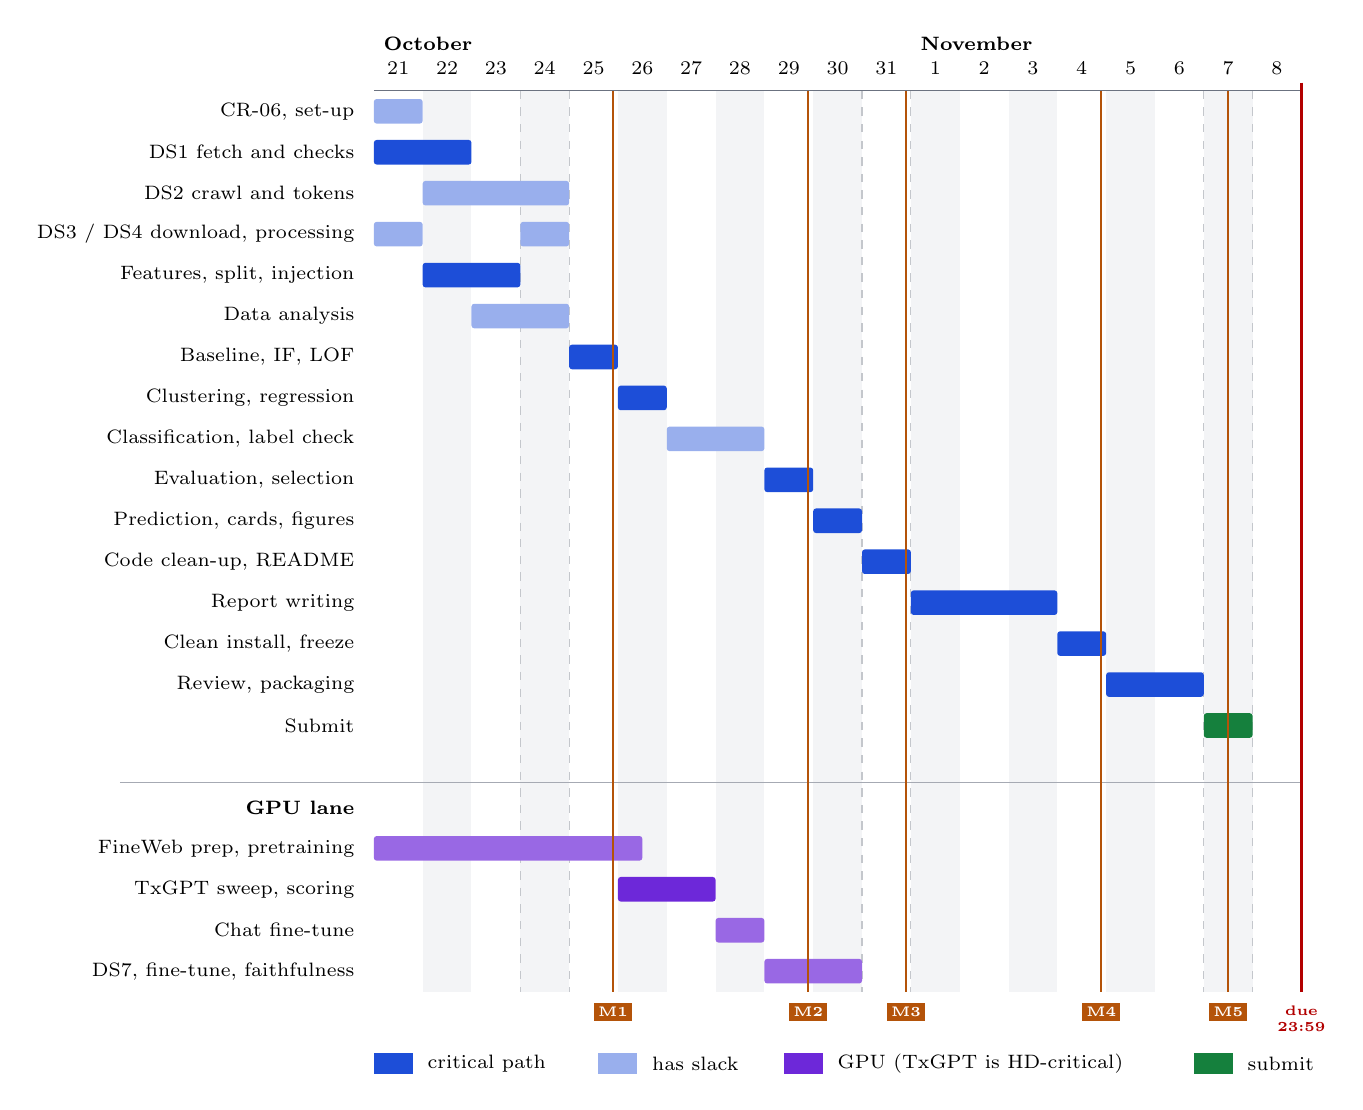
\begin{tikzpicture}[x=0.62cm, y=0.52cm, font=\scriptsize]
  % day columns: 0 = Wed 21 Oct ... 18 = Sun 8 Nov
  \def\labels{{"21","22","23","24","25","26","27","28","29","30","31","1","2","3","4","5","6","7","8"}}
  \def\nrows{22}
  \foreach \d in {0,...,18} {
    \pgfmathsetmacro{\lab}{\labels[\d]}
    \node[anchor=south] at (\d+0.5, 0.15) {\lab};
    \ifodd\d \fill[greysoft] (\d,0) rectangle (\d+1,-\nrows); \fi
  }
  \node[anchor=south west, font=\scriptsize\bfseries] at (0,0.75) {October};
  \node[anchor=south west, font=\scriptsize\bfseries] at (11,0.75) {November};
  \draw[grey] (0,0) -- (19,0);
  % weekend shading lines
  \foreach \d in {3,4,10,11,17,18} { \draw[grey!40, dashed] (\d,0) -- (\d,-\nrows); }
  % rows: label, start, end, style
  \newcommand{\task}[5]{%
    \node[anchor=east, align=right] at (-0.2, -#1+0.5) {#2};
    \fill[#5, rounded corners=1pt] (#3, -#1+0.2) rectangle (#4, -#1+0.8);
  }
  \task{1}{CR-06, set-up}{0}{1}{accent!45}
  \task{2}{DS1 fetch and checks}{0}{2}{accent}
  \task{3}{DS2 crawl and tokens}{1}{4}{accent!45}
  \task{4}{DS3 / DS4 download, processing}{0}{1}{accent!45}
  \fill[accent!45, rounded corners=1pt] (3,-4+0.2) rectangle (4,-4+0.8);
  \task{5}{Features, split, injection}{1}{3}{accent}
  \task{6}{Data analysis}{2}{4}{accent!45}
  \task{7}{Baseline, IF, LOF}{4}{5}{accent}
  \task{8}{Clustering, regression}{5}{6}{accent}
  \task{9}{Classification, label check}{6}{8}{accent!45}
  \task{10}{Evaluation, selection}{8}{9}{accent}
  \task{11}{Prediction, cards, figures}{9}{10}{accent}
  \task{12}{Code clean-up, README}{10}{11}{accent}
  \task{13}{Report writing}{11}{14}{accent}
  \task{14}{Clean install, freeze}{14}{15}{accent}
  \task{15}{Review, packaging}{15}{17}{accent}
  \task{16}{Submit}{17}{18}{okgreen}
  \draw[grey!60] (-5.2,-16.9) -- (19,-16.9);
  \node[anchor=east, align=right, font=\scriptsize\bfseries] at (-0.2,-17.5) {GPU lane};
  \task{19}{FineWeb prep, pretraining}{0}{5.5}{violet!70}
  \task{20}{TxGPT sweep, scoring}{5}{7}{violet}
  \task{21}{Chat fine-tune}{7}{8}{violet!70}
  \task{22}{DS7, fine-tune, faithfulness}{8}{10}{violet!70}
  % milestones
  \foreach \x/\m in {4.9/M1, 8.9/M2, 10.9/M3, 14.9/M4, 17.5/M5} {
    \draw[warn, thick] (\x,0) -- (\x,-\nrows);
    \node[fill=warn, text=white, font=\tiny\bfseries, inner sep=1.5pt] at (\x,-\nrows-0.5) {\m};
  }
  \draw[red!70!black, very thick] (19,0.2) -- (19,-\nrows);
  \node[anchor=north, text=red!70!black, font=\tiny\bfseries, align=center] at (19,-\nrows-0.1) {due\\23:59};
  % legend
  \begin{scope}[shift={(0,-\nrows-2.0)}]
    \fill[accent] (0,0) rectangle (0.8,0.5); \node[anchor=west] at (0.9,0.25) {critical path};
    \fill[accent!45] (4.6,0) rectangle (5.4,0.5); \node[anchor=west] at (5.5,0.25) {has slack};
    \fill[violet] (8.4,0) rectangle (9.2,0.5); \node[anchor=west] at (9.3,0.25) {GPU (TxGPT is HD-critical)};
    \fill[okgreen] (16.8,0) rectangle (17.6,0.5); \node[anchor=west] at (17.7,0.25) {submit};
  \end{scope}
\end{tikzpicture}}
\caption{A2 schedule from Wednesday 21 October to Sunday 8 November. Dashed lines mark weekends;
orange lines mark milestones M1--M5.}
\end{figure}

\subsection{Milestones and what each one proves}

\begin{center}
\small
\begin{tabularx}{\textwidth}{@{}L{1.0cm}L{2.2cm}Y@{}}
\toprule
\textbf{ID} & \textbf{Date} & \textbf{Evidence that it happened} \\
\midrule
M1 & Sun 25 Oct & \code{scores.csv} holds baseline, Isolation Forest and LOF scores for every scorable DS1 transaction (A1 Objective 2), and the DR-02 tests pass. \\
M2 & Thu 29 Oct & Every evaluation table exists. The Explorer's method is selected and recorded. Results are tagged \code{results-v1}. \\
M3 & Sat 31 Oct & Every planned function exists; notebooks run clean; tests pass; the README draft is complete. \\
M4 & Wed 4 Nov & A teammate rebuilt \fp{reports/tables/} from the README alone. The code is tagged \code{v1.0} and frozen; after this, only bug fixes go in, each logged. \\
M5 & Sat 7 Nov & The Canvas receipt is saved, and the submitted files were downloaded back and opened. \\
\bottomrule
\end{tabularx}
\end{center}

\subsection{The critical path and the slack}

The critical path is: DS1 fetch → features and split → baseline → clustering and regression →
evaluation → selection → prediction → clean-up → report → clean install → packaging → submission.
Classification on DS3 and DS4 has about one day of slack, because the report's evaluation section
doesn't need it until 2 November. The GPU lane has about three days of slack before TxGPT's
results are needed (29 October), and the text model's gate protects that slack. Sunday 8 November
is a full spare day.

\textbf{If a day slips.} First use the slack in the non-critical rows. Then drop items from the
bottom of the priority list (Section~\ref{sec:moscow}). Never touch the 7 November submission.

\section{Risks, priorities and the submission checklist}
\label{sec:risks}

\subsection{Risk register for Assignment 2}
\label{sec:riskregister}

The register continues A1's numbering, owners and scoring, so markers can follow a risk from one
report to the next. A1 risks that still matter keep their number, with the trigger rewritten for
A2. New risks start at 23. The score is likelihood × impact with A1's mapping: Unlikely 1, Low 2,
Moderate 3, Likely and High 4; impact Low 2, Medium 3, High 4, Critical 5. Rows are sorted by
score. The register is reviewed at every weekly meeting and after each milestone, and the minutes
record any change.

{\small
\begin{longtable}{@{}L{0.7cm}L{3.2cm}L{2.0cm}L{3.4cm}L{4.6cm}@{}}
\toprule
\textbf{No.} & \textbf{Risk} & \textbf{L × I} & \textbf{Trigger / owner} & \textbf{Prevention; fallback} \\
\midrule
\endhead
4 & Methods fail the label-free checks (plant recall or stability) & High × High\newline 4×4 = 16 &
Recall below 70\% for 2 of 3 patterns, or Jaccard below 0.7, at M2 (29 Oct) / Cao Tri Tran &
\textit{Prevention:} threshold sweep and separate tuning plants; the CR-02/04/05 ablation; seven
candidate methods instead of three. \textit{Fallback:} the selection rule picks the best stable
method, even if that is the baseline; the report explains the miss (Section~\ref{sec:evaluation}). \\
9 & Code doesn't run on the marker's machine & Likely × High\newline 4×4 = 16 &
The M4 clean install fails or needs help / Le Quang Anh Hoang &
\textit{Prevention:} CPU-only \code{environment.yml} with pinned versions; \code{requirements.txt};
offline rebuild; \code{pathlib} paths; tests as the quick check. \textit{Fallback:} README
troubleshooting with expected output pasted in; contact the tutor at once. \\
7 & Critical-path tasks slip & Moderate × Critical\newline 3×5 = 15 &
A critical-path row ends a day late, or DS1 isn't fetched by the end of 21 Oct / Le Quang Anh Hoang &
\textit{Prevention:} DS1 starts on day 37; a daily check against Section~\ref{sec:schedule}; the
GPU lane is off the critical path. \textit{Fallback:} use slack, then cut from the bottom of the
priority list (Section~\ref{sec:moscow}). The 7 November submission never moves. \\
6 & Scope creep: HD extras eat time that Must items need & Likely × Medium\newline 4×3 = 12 &
Work on a Should or Could item while a Must item is behind / Le Quang Anh Hoang &
\textit{Prevention:} the priority list; the pretraining gate; GPU jobs run unattended.
\textit{Fallback:} stop the item and record the cut in the minutes. \\
13 & Unsupported claims about real transactions & Moderate × High\newline 3×4 = 12 &
Reworded by D-A2-3: any draft claims precision, recall, F1 or accuracy for real snapshot
transactions / Cao Tri Tran &
\textit{Prevention:} the metrics rule (Section~\ref{sec:metricsrule}); ``against the dataset's
labels'' wording; banned-word scan; number-check script. \textit{Fallback:} delete the claim and
restate it as a ranking with limitations. \\
23 & Pretraining is slower than estimated, or is interrupted & Likely × Medium\newline 4×3 = 12 &
The benchmark projects more than 72 h for 2B tokens, or a run stops overnight / Cao Tri Tran &
\textit{Prevention:} the gate (Section~\ref{sec:gate}); checkpoints every 30 minutes; Windows
Update paused; resume already tested. \textit{Fallback:} cut tokens to the measured budget (floor
1B); below the floor, TxGPT is the only language model, as CR-06 records. \\
26 & The small text model writes wrong numbers or banned words & High × Medium\newline 4×3 = 12 &
Raw number faithfulness below 95\% on the DS7 test set / Cao Tri Tran &
\textit{Prevention:} the guardrail; the template is authoritative; five phrasings per template in
DS7. \textit{Fallback:} \code{use_assistant=False} stays the default; the report gives raw and
guarded rates. \\
30 & A bug found after the results freeze changes numbers & Moderate × High\newline 3×4 = 12 &
A test failure or review finding after M2 / Cao Tri Tran &
\textit{Prevention:} tests green before M2; tables generated, never typed; report numbers checked
by script. \textit{Fallback:} fix, re-run \code{all --offline} (under an hour on CPU), regenerate
tables, log it in \code{CHANGELOG.md}. \\
31 & Generative-AI use undeclared or under-declared & Low × Critical\newline 2×5 = 10 &
No declaration drafted by 5 Nov / Cam Dan Bui &
\textit{Prevention:} the declaration is a listed submission file; a running log of what AI helped
with, kept from today. \textit{Fallback:} ask the tutor how to add it if it was missed. \\
2 & A dataset is unavailable or its licence is unclear & Moderate × Medium\newline 3×3 = 9 &
Elliptic's Kaggle licence not confirmed by 24 Oct, or a download fails / Cao Tri Tran &
\textit{Prevention:} download on 21 Oct; record each licence; ship a script and checksums when
redistribution is unclear. \textit{Fallback:} BitcoinHeist (CC BY 4.0) carries the classification
alone; the Elliptic++ transaction set is the substitute. \\
5 & A teammate can't do their review task in time & Moderate × Medium\newline 3×3 = 9 &
Manifest review (22 Oct), code review (24--25 Oct), ratings (2 Nov), clean install (4 Nov) or
proofread (5 Nov) late / Le Quang Anh Hoang &
\textit{Prevention:} every task has a name and a date in the CR-06 message, plus a named backup.
\textit{Fallback:} the backup does it; otherwise the report says who did the check, or that it
was not done. \\
15 & Esplora rate limits block DS1 or DS2 & Moderate × Medium\newline 3×3 = 9 &
More than 5\% of requests return 429 in an hour, or DS2 has under 3,000 addresses by 23 Oct / Le
Quang Anh Hoang &
\textit{Prevention:} pacing, back-off, caching, a resumable state file, the mempool.space fallback,
overnight crawling. \textit{Fallback:} accept the 3,000 floor and say so; a second crawl night
uses DS2's slack. \\
19 & Sample selection bias & Moderate × Medium\newline 3×3 = 9 &
No written rule in the manifest before fetching / Cao Tri Tran &
\textit{Prevention:} the rule is fixed and seeded first, and every skip is logged.
\textit{Fallback:} a limitations paragraph states the bias. \\
22 & The prototype promises what A2 can't deliver & Moderate × Medium\newline 3×3 = 9 &
\code{predict.py} output differs from the shapes in \code{types.ts} / Minh Khang Nguyen &
\textit{Prevention:} \code{test_predict.py} checks every shape. \textit{Fallback:} update the
prototype through change control. \\
24 & Out of memory or disk & Moderate × Medium\newline 3×3 = 9 &
Under 40 GB free on 21 Oct, swapping during random-forest tuning, or CUDA out of memory / Cao Tri Tran &
\textit{Prevention:} memory-mapped tokens; \code{--delete-raw}; capped \code{n_jobs}; heavy CPU jobs
never overlap. \textit{Fallback:} micro-batch 4 with more accumulation (same effective batch);
\code{n_jobs=4}; raw shards on an external disk. \\
27 & TxGPT doesn't beat the habit or Markov baselines & Moderate × Medium\newline 3×3 = 9 &
Test NLL no lower than the address-habit baseline at M2 / Cao Tri Tran &
\textit{Prevention:} the size sweep with 3 seeds; DS2 stretch target of 10,000 addresses.
\textit{Fallback:} report it as a finding. It is still a valid experiment, but TxGPT is then not
the Explorer's method. \\
28 & The zip exceeds Canvas's upload limit & Moderate × Medium\newline 3×3 = 9 &
The 1 Nov dry-run zip is over the confirmed limit / Le Quang Anh Hoang &
\textit{Prevention:} the limit checked on 22 Oct; DS2 in Parquet; fp16 weights. \textit{Fallback:}
the Assistant weights and Elliptic move to a link with SHA-256, and the README says where. \\
29 & The report goes over 3,000 words, or tables count & Moderate × Medium\newline 3×3 = 9 &
Body above 2,850 words on 3 Nov, or the tutor says tables count / Cam Dan Bui &
\textit{Prevention:} the word budget per section (Section~\ref{sec:report}); lean tables; detail in
appendices. \textit{Fallback:} move tables to appendices; trim §7.1 and §2 first. \\
14 & Data leakage inflates results & Low × High\newline 2×4 = 8 &
Results unexpectedly strong (Elliptic far above Weber et al.\ 2019; random split far above the
temporal split), or a DR-02 test fails / Cao Tri Tran &
\textit{Prevention:} the leakage controls (Section~\ref{sec:leakage}) and tests; the test period is
used once. \textit{Fallback:} rebuild, re-run, replace the numbers, log it. \\
16 & Real addresses read as accusations, or terms forbid a use & Low × High\newline 2×4 = 8 &
Any text implies wrongdoing by a DS1 or DS2 address, or a licence forbids the planned use / Le
Quang Anh Hoang &
\textit{Prevention:} hashed DS2 IDs with the salt kept out of the zip; the limitation line; no
labels attached to real addresses; licences recorded. \textit{Fallback:} shorten or replace IDs;
drop the dataset. \\
25 & CR-06 is rejected or the answer is delayed & Low × High\newline 2×4 = 8 &
No tutor reply by 23 Oct, or a ``no'' / Cam Dan Bui &
\textit{Prevention:} sent on 20--21 Oct; the plan builds every reading (all three types, IF and LOF,
both language models), so almost any answer is already covered. \textit{Fallback:} continue on
the plan's reading, which meets the brief's literal text; record the open question in the
minutes; adjust only the report's framing. \\
10 & Upload or naming error causes a late penalty & Unlikely × Medium\newline 1×3 = 3 &
Not submitted 24 hours before the deadline / Le Quang Anh Hoang &
\textit{Prevention:} the checklist in Section~\ref{sec:checklist}; submit on 7 Nov.
\textit{Fallback:} resubmit at once; if past the deadline, tell the tutor and submit anyway. \\
\bottomrule
\end{longtable}
}

\textbf{A1 risks not carried forward:} 1 (now covered by 4 and the threshold sweep), 3 (an A3
usability question), 8 (A1's demo video), 11 (the team handles minutes separately), 12 (covered by
13 and 16), 17 (D1 passed), 18 (the amount derivation is tested; still checked in DS1's sums), 20
(resolved) and 21 (the Confluence trial ended on 15 October, so the change log now lives in the
repository as \code{docs/change-log.md}).

\subsection{Early-warning signals}

Most of these risks show up early if someone looks. Each signal below takes under a minute to
check, and the morning check runs every day from 21 October to 7 November.

\begin{center}
\small
\begin{tabularx}{\textwidth}{@{}L{3.9cm}L{3.6cm}Y@{}}
\toprule
\textbf{Signal} & \textbf{Threshold} & \textbf{Action} \\
\midrule
GPU tokens per second against the benchmark & 15\% lower & Check temperature and other GPU use; restart from the checkpoint if speed doesn't recover (risk 23). \\
Pretraining validation loss after warm-up & No fall over 3 evaluations & Inspect \code{log.jsonl}; check the learning rate and the data order before spending more GPU hours. \\
GPU temperature & Above 83 °C & Improve airflow; lower the power limit in the NVIDIA settings if needed. \\
Crawl 429 rate & Above 5\% over an hour & Slow the pace to 1 s; switch to mempool.space for an hour (risk 15). \\
Free disk space & Below 15 GB & Delete used FineWeb shards and old checkpoints, keeping \code{ckpt_last.pt} and \code{model_best.pt} (risk 24). \\
Critical-path row & Not done by the end of its day & Re-plan the next morning; cut from the priority list (risk 7). \\
Test suite & Any failure & Stop new features until it is green again (risk 30). \\
Section word count while drafting & Over its budget & Trim the same day (risk 29). \\
\bottomrule
\end{tabularx}
\end{center}

\subsection{Priority list}
\label{sec:moscow}

The list decides what gets cut if time runs short. \textbf{Must} items give a complete
submission and keep A1's promises; they are never cut, only shrunk (fewer grid points, a smaller
DS2). \textbf{Should} items earn the HD points. \textbf{Could} items are done only with spare
time. \textbf{Won't} items are named so nobody starts them.

\begin{center}
\small
\begin{tabularx}{\textwidth}{@{}L{1.2cm}Y L{3.4cm}@{}}
\toprule
\textbf{ID} & \textbf{Item} & \textbf{Earns} \\
\midrule
\multicolumn{3}{@{}l}{\textbf{Must}} \\
M-1 & DS1 snapshot, checks and manifest & Report 1; Code 2; A1 Obj.\ 1 \\
M-2 & Cleaning, F1--F4, the time split and the DR-02 tests & Report 1; Code 1 \\
M-3 & Baseline, Isolation Forest and LOF scoring every transaction & A1 Obj.\ 2; Code 1 \\
M-4 & K-Means and DBSCAN; regression models & Brief's model types; Code 1 \\
M-5 & Classification on DS3 (on DS4 if DS3's licence blocks it) & Brief's metrics; Code 1 \\
M-6 & Evaluation suite, method selection, objectives table & Code 1; Report 6 \\
M-7 & \code{predict.py} and the prediction CLI & Code 3 \\
M-8 & README, docstrings, package structure, data card & Code 2--5 \\
M-9 & The report, the zip and the AI declaration & Report 1--6 \\
\midrule
\multicolumn{3}{@{}l}{\textbf{Should} (if cuts are needed, cut from the bottom of this list up)} \\
S-1 & DS2 crawl and TxGPT (the tutor's language-model requirement) & HD ML; HD datasets \\
S-2 & DS4 BitcoinHeist, with all three split schemes & HD datasets \\
S-3 & The label check on DS3 and DS4 & HD ML; Report 2 \\
S-4 & Reviewer check (A1 promise; depends on two teammates) & Report 7.2 \\
S-5 & Text-model pretraining and chat fine-tune & HD ML; HD datasets \\
S-6 & DS7, the explanation fine-tune and the guardrail & HD ML; A3 \\
S-7 & Address-profile clustering on DS1 and DS2 & Report 2; A3 \\
S-8 & A model card per final model & Code 2 \\
\midrule
\multicolumn{3}{@{}l}{\textbf{Could}} \\
C-1 & DS9: score Ransomwhere addresses with our own pipeline & HD datasets \\
C-2 & DS8: address-level classification on Elliptic++ actors & HD datasets \\
C-3 & Multi-class family classification on DS4 & HD ML \\
C-4 & ``Flag if either method flags'' as an option for A3 & A3 \\
C-5 & A TxGPT ablation with finer amount buckets & HD ML \\
\midrule
\multicolumn{3}{@{}l}{\textbf{Won't} (in A2)} \\
W-1 & Graph neural networks on Elliptic & future work \\
W-2 & Live API calls from the Explorer & A1 scope rule \\
W-3 & Fine-tuning a public pretrained model & tutor's rule \\
W-4 & Ethereum or other chains; XGBoost or LightGBM & scope; dependencies \\
W-5 & Whole-chain datasets (ORBITAAL, the Bitcoin temporal graph) & 16 GB RAM; schedule \\
\bottomrule
\end{tabularx}
\end{center}

\textbf{Cut order if a day is lost:} C-5, C-4, C-3, C-2, C-1, then S-8, S-7, S-6, S-5. Cutting
S-5 leaves TxGPT as the only language model, which the tutor question in CR-06 prepares for. S-4
is cut only if the teammates can't do it. S-1 is cut last because it is the HD-critical model.

\subsection{Submission checklist}
\label{sec:checklist}

Run on 6 November (build) and 7 November (submit). Every line is ticked by the named person,
and the finished list is pasted into that week's minutes.

{\small
\begin{longtable}{@{}L{8.6cm}L{2.8cm}L{2.6cm}@{}}
\toprule
\textbf{Check} & \textbf{Who} & \textbf{When} \\
\midrule
\endhead
\multicolumn{3}{@{}l}{\textbf{Report PDF}} \\
Named \fp{HCMC_COS30049.1_4_Assignment2_Report.pdf}; opens; fonts embedded & Cao Tri Tran & 6 Nov \\
Cover has the group name and ID, four names and IDs, \textbf{the tutor's name}, the date and the word count & Cam Dan Bui & 5 Nov \\
Body at most 3,000 words (\code{tools/wordcount.py}); the counting rule is stated & Cao Tri Tran & 3 and 6 Nov \\
Every section the brief requires is present (Section~\ref{sec:report} checklist) & Cam Dan Bui & 5 Nov \\
Every figure and table is referenced in the text; captions say what to notice & Cam Dan Bui & 5 Nov \\
Citation check clean: nothing cited but unlisted, nothing listed but uncited & Cao Tri Tran & 6 Nov \\
Number check clean: every number matches \fp{reports/tables/} & Cao Tri Tran & 6 Nov \\
Banned-word scan clean for the tool and DS1 & Cao Tri Tran & 6 Nov \\
\multicolumn{3}{@{}l}{\textbf{Code zip}} \\
Built from tag \code{v1.0} by the packaging script & Cao Tri Tran & 6 Nov \\
\code{SHA256SUMS.txt} verifies every file & Cao Tri Tran & 6 Nov \\
Unzipped into an empty folder: \code{python -m pytest -q} passes and one prediction command runs & Le Quang Anh Hoang & 6 Nov \\
Contains README (\code{.md} and \code{.pdf}), \code{DATA_CARD.md}, \code{MODEL_CARD.md}, \code{LICENSES.md} & Cao Tri Tran & 6 Nov \\
Contains no salt, \code{.git}, caches, raw FineWeb or unused data & Cao Tri Tran & 6 Nov \\
Size under Canvas's limit; anything linked has a SHA-256 in the README & Le Quang Anh Hoang & 6 Nov \\
\multicolumn{3}{@{}l}{\textbf{Prepared by the team separately}} \\
Meeting minutes for every week since the team formed (W1--W8), including CR-06's approval and the reviews & Cam Dan Bui & 6 Nov \\
Contribution form signed by all four members & All & 6 Nov \\
\multicolumn{3}{@{}l}{\textbf{Declaration and upload}} \\
AI declaration: what AI helped with, and that the team checked and owns the work & Cam Dan Bui & 5 Nov \\
All five files uploaded on Canvas by one member & Le Quang Anh Hoang & 7 Nov \\
Canvas receipt saved; the submitted files downloaded back and opened & Le Quang Anh Hoang & 7 Nov \\
\bottomrule
\end{longtable}
}

\subsection{After submission: what Assignment 3 inherits}

\begin{itemize}
  \item The tag \code{v1.0} and the frozen \fp{reports/tables/}. A3 builds on them without changing
    A2's numbers.
  \item \code{explorer/predict.py} and its JSON shapes, which the FastAPI back end wraps directly.
  \item The guarded Explorer Assistant, which is optional in A3 and off by default.
  \item The usability walkthrough (A1 team action T7) and the A3 user study, which reuse A1's
    observer sheet.
  \item A short lessons-learned note in the Week 9 minutes: what took longer than planned, and why.
\end{itemize}


\appendix
\section{Change request CR-06 and the messages to send}
\label{app:cr06}

A1 §8.5 requires a change request to change a must-have item, add or remove a work package,
change acceptance criteria, or use more than half of an assignment buffer. CR-06 does all four,
so it needs every member's approval. It also touches the brief's marking requirements, so the
tutor sees it before work depends on it.

\subsection{Change log entry}

The fields follow A1's Change Log (ID, date, requestor, proposal, impact, decision, approvers,
changed artifacts). The Confluence trial ended on 15 October (A1 risk 21), so from CR-06 onwards
the log lives in the repository as \code{docs/change-log.md}, with CR-01 to CR-05 copied in from
the exported CSV.

\begin{center}
\small
\begin{tabularx}{\textwidth}{@{}L{3.0cm}Y@{}}
\toprule
\textbf{Field} & \textbf{Entry} \\
\midrule
ID & CR-06 \\
Date raised & Tuesday 20 October 2026 \\
Requestor & Cao Tri Tran (Data/ML Lead) \\
Proposal & Adopt decisions D-A2-1 to D-A2-5 (Section~\ref{sec:decisions}): (1) cover clustering, regression and classification, keeping the baseline, Isolation Forest and LOF as extras; (2) add datasets DS2--DS7, with DS8 and DS9 optional; (3) report label-based metrics only where labels exist; (4) train two language models from scratch; (5) one repository with a CPU environment for markers and a GPU environment for retraining. \\
Reason & The A2 brief requires at least two of three named model types and reports accuracy, precision, recall and F1. A1's two outlier detectors may not count as two types, and A1's single unlabelled dataset can't support those metrics honestly. The HD band rewards additional datasets and additional ML implementations, and the tutor asked for a locally trained language model. \\
Impact on scope & Must items are added (clustering, regression, classification, prediction interface). Nothing A1 promised is removed: every A1 method and check is still delivered (Section~\ref{sec:a1promises}). \\
Impact on schedule & A1's baseline put WBS 1.2.1 on 11--13 October; it now starts on 21 October. The new schedule (Section~\ref{sec:schedule}) runs four lanes in parallel and still submits a day early, but it uses more than half of the A2 buffer. \\
Impact on risk & Risk 13's trigger is reworded (Section~\ref{sec:metricsrule}). New risks 23--31 are added (Section~\ref{sec:riskregister}). \\
Impact on quality & More evidence: three labelled-data experiments, a reviewer check, a clean-install test and two model cards. \\
Cost & No money. About 70--90 hours of GPU time on the Data/ML Lead's own PC (Section~\ref{sec:compute}), and its electricity. \\
Decision & \textit{Pending}: approved, approved with changes, or rejected. \\
Approvers & Cam Dan Bui; Cao Tri Tran; Le Quang Anh Hoang; Minh Khang Nguyen. The tutor is informed. \\
Changed artifacts & WBS and WBS dictionary (1.2.1--1.2.8), schedule baseline (v2), risk register, requirements DR-01 and DR-02 (wording only), \code{settings.json}. \\
\bottomrule
\end{tabularx}
\end{center}

\subsection{Effect on the A1 work breakdown}

Durations are A1's planned working days. The owners stay as A1 named them (Cam Dan Bui and Cao
Tri Tran for every 1.2 package), except the new 1.2.8.

\begin{center}
\small
\begin{tabularx}{\textwidth}{@{}L{3.6cm}C{1.2cm}Y@{}}
\toprule
\textbf{Package (A1 code)} & \textbf{A1 days} & \textbf{Change under CR-06} \\
\midrule
1.2.1 Build data snapshot & 3 & Also: the DS2 crawl, the DS3 and DS4 downloads, and DS5--DS6 preparation. DS1 itself is unchanged. \\
1.2.2 Clean data and build features & 4 & Also: the DS3 join and temporal split, DS4 transforms and sampling, TxGPT tokenisation, the refinement ablation. \\
1.2.3 Explore and visualise & 3 & Also: the labelled-data analyses and the DS2 checks (Section~\ref{sec:analysis}). \\
1.2.4 Build baseline and models & 5 & Now all three model types plus the A1 extras (Section~\ref{sec:models}). \\
1.2.5 Evaluate and select & 3 & Also: labelled-data metrics, the label check and the language-model evaluation. A1's selection rule is unchanged. \\
1.2.6 Code, README and zip & 2 & Also: \code{predict.py}, the data and model cards, and the M4 clean install. \\
1.2.7 Write report & 4 & Same 3,000-word limit; the content follows Section~\ref{sec:report}. \\
\textbf{1.2.8 Language models (new)} & -- & TxGPT and the Explorer Assistant on the GPU lane, in parallel with 1.2.2--1.2.5, about 3 days of float. Owner: Cao Tri Tran. Done when both models are trained, evaluated and exported (Section~\ref{sec:lm}). \\
\bottomrule
\end{tabularx}
\end{center}

\subsection{Approval steps}

\begin{enumerate}
  \item \textbf{20 October.} Post the team message below in Discord, with this plan's PDF attached.
  \item \textbf{By 21 October, 12:00.} Each member replies ``approve'' or states an objection.
    An objection is discussed in a call that evening; nothing waits longer than that.
  \item \textbf{21 October.} Send the tutor message below. Work that doesn't depend on the answers
    (DS1, features, the baseline) carries on meanwhile.
  \item Record the decision, approvers and date in \code{docs/change-log.md}, and save the
    schedule as baseline v2.
  \item The Week 6 minutes record the approval with names and dates, and the tutor's answers
    when they arrive.
\end{enumerate}

\subsection{Message to the tutor}

\begin{summarybox}
\small
\textbf{Subject:} COS30049 HCMC\_COS30049.1\_4: Assignment 2 approach and four quick questions

Dear \textit{<tutor's name>},

Our Assignment 1 plan used outlier detectors (Isolation Forest and LOF) on an unlabelled Bitcoin
snapshot. To meet the Assignment 2 brief, we plan to:
\begin{itemize}[leftmargin=*]
  \item add clustering (K-Means, DBSCAN) and regression on our own snapshot, and classification on
    two labelled public datasets (Elliptic and BitcoinHeist), keeping Isolation Forest and LOF as
    additional experiments;
  \item report accuracy, precision, recall and F1 only against those datasets' own labels, never
    for our unlabelled snapshot;
  \item train two language models from scratch on our own GPU: TxGPT, a small transformer over
    sequences of Bitcoin transactions, and a 152M-parameter text model that explains flags in
    plain language. Neither starts from anyone else's weights.
\end{itemize}

Could you confirm four things?
\begin{enumerate}[leftmargin=*]
  \item Does this mapping meet ``at least two types of machine learning models''?
  \item Does TxGPT on its own satisfy the language-model requirement for HD, or do you expect a
    text model as well?
  \item Do tables and captions count towards the 3,000 words?
  \item What is the Canvas upload limit for the zip? If the text model's weights (about 305 MB)
    are too large, may we link them with a checksum instead? The same question applies to the
    Elliptic data if its licence doesn't allow redistribution.
\end{enumerate}

We will include a generative-AI declaration as you asked. If there is a template, we will use it.

Kind regards,\\
Cao Tri Tran, for HCMC\_COS30049.1\_4
\end{summarybox}

\subsection{Message to the team}

\begin{summarybox}
\small
\textbf{CR-06 (A2 plan): please approve by Wednesday 12:00.} Full plan attached. In short: we add
clustering, regression and classification so A2 meets the brief's model-type rule; we add
labelled datasets (Elliptic, BitcoinHeist) for honest precision and recall; and I train two
language models from scratch on my GPU for HD. Every A1 promise is still delivered.

What I need from each of you, with dates:
\begin{itemize}[leftmargin=*]
  \item \textbf{Cam Dan Bui:} DS1 manifest review and one manual transaction check (22 Oct);
    reviewer ratings (29 Oct to 2 Nov); rubric review and proofread (5 Nov); the AI declaration
    draft (5 Nov). Also: what is our tutor's full name for the cover?
  \item \textbf{Le Quang Anh Hoang:} code review of \code{features.py}, \code{split.py} and
    \code{inject.py} (24--25 Oct); clean install from the README on a fresh Windows machine
    (4 Nov); Canvas upload (7 Nov).
  \item \textbf{Minh Khang Nguyen:} reviewer ratings (29 Oct to 2 Nov); check that
    \code{predict.py}'s output still fits the prototype's screens (30 Oct).
  \item \textbf{Everyone:} minutes for Weeks 1--8 and the contribution form, by 6 Nov.
\end{itemize}
Reply ``approve'' or tell me what to change.
\end{summarybox}

\section{Datasets considered}
\label{app:datasets}

The HD criterion rewards a ``large number of additional datasets'', but only datasets that a
final model uses go in the zip, and each one costs collection, processing and report words. So
the candidates were checked against four tests: is it Bitcoin, does it carry labels we can use
honestly, is its licence clear, and does it fit a 16 GB machine and a 19-day schedule. The
datasets in use are DS1--DS9 (Section~\ref{sec:datasets}). The table below lists the eighteen
others, checked on 20 October 2026, with the decision for each. It also repeats DS9, the
optional Ransomwhere set, so its reasoning sits beside the rest.

\textbf{Decisions:} \emph{Fallback} means it replaces a chosen dataset if that one fails;
\emph{Could} means it is on the priority list's Could tier; \emph{Not used} means it fails one of
the four tests; \emph{Won't} means it is ruled out for A2 (Section~\ref{sec:moscow}).

{\small
\begin{longtable}{@{}L{3.1cm}L{4.4cm}L{2.4cm}L{4.4cm}@{}}
\toprule
\textbf{Dataset (source)} & \textbf{What it holds} & \textbf{Licence and access} & \textbf{Decision and reason} \\
\midrule
\endhead
\multicolumn{4}{@{}l}{\textbf{Bitcoin, labelled}} \\
Elliptic++ transactions (Elmougy and Liu 2023) & Elliptic's transactions with 183 features and the same labels; also wallet-level (actor) files with 56 features & None stated; Google Drive link from the GitHub README & \emph{Fallback} for DS3 if Elliptic's Kaggle licence blocks it. The actor files are DS8. \\
Elliptic2 (Bellei et al.\ 2024) & 122,000 labelled subgraphs inside a background graph of 49M node clusters and 196M edges & Code Apache 2.0; data licence not stated; download via Elliptic's website & \emph{Not used.} Subgraph labels need graph neural networks (W-1), and the background graph is too large for 16 GB of RAM. \\
BABD-13 (Xiang et al.\ 2024) & 544,462 labelled addresses of 13 behaviour types, 148 features, July 2019 to May 2021 & Host and licence not confirmed & \emph{Not used} unless a confirmed copy appears. It would be a third classification set with little new to say, and its features need a subgraph tool we would have to rebuild. \\
Ransomwhere (Cable 2024) & Crowdsourced ransomware payment addresses with transactions and family; 5.6 MB JSON & CC BY 4.0; Zenodo & \emph{Could}, as DS9. Its addresses run through our own pipeline, which gives a label check in our own feature space. \\
Showing the Receipts (GitHub, \code{cablej}) & 1,013 likely ransomware payment addresses & CC BY 4.0 & \emph{Not used.} Same purpose as Ransomwhere but smaller; kept as a cross-check if DS9 runs. \\
Ransomware seed addresses (Paquet-Clouston, Haslhofer and Dupont 2019) & Seed address CSV, with an expanded set on Zenodo & No licence file & \emph{Not used.} No licence, and it overlaps DS4's label sources. \\
OFAC sanctioned addresses (GitHub, \code{0xB10C}) & Bitcoin addresses on the US sanctions list, regenerated nightly & Repository licence not stated & \emph{Won't.} A ``sanctioned'' label on real addresses is an identity claim, which A1 risk 16 rules out. \\
Bitcoin Ponzi addresses (Bartoletti, Pes and Serusi 2018) & Addresses of Ponzi schemes with features & Host and size not found & \emph{Not used.} No confirmed download. \\
WalletExplorer entity labels & Exchanges, pools and services found by co-spend clustering & No bulk download or licence & \emph{Not used.} No licence; research reports stale names. \\
\multicolumn{4}{@{}l}{\textbf{Bitcoin, whole chain or graph}} \\
ORBITAAL (Coquidé and Cazabet 2024) & Entity-level temporal graph, January 2009 to January 2021 & CC BY 4.0; Zenodo; 156.9 GB & \emph{Won't} (W-5): size. \\
Bitcoin temporal graph (Schnoering and Vazirgiannis 2024) & 252M entity nodes, 786M edges, 34,098 labelled entities & CC BY 4.0; Figshare; PostgreSQL, about 120 GB & \emph{Won't} (W-5): size. Good future work for address profiles. \\
BigQuery \code{crypto_bitcoin} (Google public dataset) & The whole chain as SQL tables & First 1 TB of queries a month free; needs a Google Cloud project & \emph{Fallback} for the DS2 crawl if Esplora blocks it. \\
Blockchair database dumps & Blocks, transactions and outputs as TSV & Licence not confirmed & \emph{Not used.} Licence unclear; Esplora covers the need. \\
SNAP Bitcoin Alpha (Kumar et al.\ 2016) & 3,783 traders, 24,186 trust ratings from $-10$ to $+10$ & Public download from SNAP & \emph{Not used.} Trust ratings between traders, not transactions. \\
\multicolumn{4}{@{}l}{\textbf{Not Bitcoin}} \\
IBM AML (Altman et al.\ 2023) & Synthetic bank transfers with an ``Is Laundering'' label, in six sizes & Kaggle; licence not confirmed & \emph{Not used.} Bank transfers, not Bitcoin. \\
SAML-D (Oztas et al.\ 2023) & About 9.5M synthetic monitored transactions, 12 features, 28 typologies & Kaggle; licence not confirmed & \emph{Not used.} Same reason. \\
SynthAML (Jensen et al.\ 2023) & 20,000 bank alerts (17\% reported) and over 16M transactions & Figshare; data licence not explicit & \emph{Not used.} Same reason. \\
Ethereum fraud sets (Kaggle, XBlock, Forta) & Labelled Ethereum accounts, for example 9,841 accounts with 22\% flagged & Varies & \emph{Won't} (W-4): outside A1's Bitcoin scope. \\
Card-fraud sets (ULB credit card, PaySim, Sparkov) & Card or mobile payments with fraud labels & Varies & \emph{Not used.} Not Bitcoin. \\
\bottomrule
\end{longtable}
}

\textbf{How the report uses this.} One sentence in the data-collection section, ``Eighteen other
public datasets were assessed against four criteria (Appendix~X)'', plus this table condensed in
the report's appendix. That shows selection, which the HD band and data criterion reward, at no
cost to the word limit. Entries that the report names must be cited (the second list in
Appendix~\ref{app:refs}). Details marked ``not confirmed'' are checked again before they appear
in the report.

\section{Draft reference list}
\label{app:refs}

This is the starting list for the report's bibliography, in A1's numbered Harvard style:
alphabetical, numbered, with author--date citations in the text. The report keeps only the
entries it actually cites, and the citation script (Section~\ref{sec:report}) checks that.

\textbf{How far each entry is checked.}
\textdagger\ means the details were confirmed on the source page on 20 October 2026.
\textdaggerdbl\ means the entry is copied from A1's reference list, which was checked for A1.
Unmarked entries were written from the published record and must be checked against their DOI
or source page before the report uses them. Entries with more than four authors are shortened
to ``et al.''; expand them if Swinburne's Harvard guide asks for every author.

\subsection*{Main list}

\begin{references}
\item Akcora, C.G., Li, Y., Gel, Y.R. and Kantarcioglu, M. (2020) ‘BitcoinHeist: topological data analysis for ransomware prediction on the Bitcoin blockchain’, \textit{Proceedings of the Twenty-Ninth International Joint Conference on Artificial Intelligence (IJCAI-20)}, pp. 4439–4445. doi: 10.24963/ijcai.2020/612.

\item Ben Allal, L. et al. (2025) ‘SmolLM2: when smol goes big -- data-centric training of a small language model’, \textit{arXiv preprint}, arXiv:2502.02737. Available at: \url{https://arxiv.org/abs/2502.02737} (Accessed: 20 October 2026). \textdagger

\item Blockstream (n.d.) \textit{Esplora HTTP API}. Available at: \url{https://github.com/Blockstream/esplora/blob/master/API.md} (Accessed: 29 September 2026). \textdaggerdbl

\item Breiman, L. (2001) ‘Random forests’, \textit{Machine Learning}, 45(1), pp. 5–32. doi: 10.1023/A:1010933404324.

\item Breunig, M.M., Kriegel, H.-P., Ng, R.T. and Sander, J. (2000) ‘LOF: identifying density-based local outliers’, \textit{Proceedings of the 2000 ACM SIGMOD International Conference on Management of Data}, pp. 93–104. doi: 10.1145/342009.335388. \textdaggerdbl

\item Caliński, T. and Harabasz, J. (1974) ‘A dendrite method for cluster analysis’, \textit{Communications in Statistics}, 3(1), pp. 1–27. doi: 10.1080/03610927408827101.

\item Cohen, J. (1960) ‘A coefficient of agreement for nominal scales’, \textit{Educational and Psychological Measurement}, 20(1), pp. 37–46. doi: 10.1177/001316446002000104.

\item Conti, M., Gangwal, A. and Ruj, S. (2018) ‘On the economic significance of ransomware campaigns: a Bitcoin transactions perspective’, \textit{Computers \& Security}, 79, pp. 162–189. doi: 10.1016/j.cose.2018.08.008. \emph{(One of BitcoinHeist's label sources; confirm against Akcora et al.\ 2020 which three studies it names.)}

\item Cover, T. and Hart, P. (1967) ‘Nearest neighbor pattern classification’, \textit{IEEE Transactions on Information Theory}, 13(1), pp. 21–27. doi: 10.1109/TIT.1967.1053964.

\item Cox, D.R. (1958) ‘The regression analysis of binary sequences’, \textit{Journal of the Royal Statistical Society: Series B}, 20(2), pp. 215–242. doi: 10.1111/j.2517-6161.1958.tb00292.x.

\item Davies, D.L. and Bouldin, D.W. (1979) ‘A cluster separation measure’, \textit{IEEE Transactions on Pattern Analysis and Machine Intelligence}, PAMI-1(2), pp. 224–227. doi: 10.1109/TPAMI.1979.4766909.

\item Elliptic (2019) \textit{Elliptic Data Set} [Dataset]. Kaggle. Available at: \url{https://www.kaggle.com/datasets/ellipticco/elliptic-data-set} (Accessed: \textit{date of download}).

\item Elmougy, Y. and Liu, L. (2023) ‘Demystifying fraudulent transactions and illicit nodes in the Bitcoin network for financial forensics’, \textit{Proceedings of the 29th ACM SIGKDD Conference on Knowledge Discovery and Data Mining}. doi: 10.1145/3580305.3599803. \textdagger\ \textdaggerdbl

\item Ester, M., Kriegel, H.-P., Sander, J. and Xu, X. (1996) ‘A density-based algorithm for discovering clusters in large spatial databases with noise’, \textit{Proceedings of the Second International Conference on Knowledge Discovery and Data Mining (KDD-96)}, pp. 226–231.

\item Friedman, J.H. (2001) ‘Greedy function approximation: a gradient boosting machine’, \textit{The Annals of Statistics}, 29(5), pp. 1189–1232. doi: 10.1214/aos/1013203451.

\item Gebru, T., Morgenstern, J., Vecchione, B., Vaughan, J.W., Wallach, H., Daumé III, H. and Crawford, K. (2021) ‘Datasheets for datasets’, \textit{Communications of the ACM}, 64(12), pp. 86–92. doi: 10.1145/3458723.

\item Harris, C.R. et al. (2020) ‘Array programming with NumPy’, \textit{Nature}, 585, pp. 357–362. doi: 10.1038/s41586-020-2649-2.

\item Hoerl, A.E. and Kennard, R.W. (1970) ‘Ridge regression: biased estimation for nonorthogonal problems’, \textit{Technometrics}, 12(1), pp. 55–67. doi: 10.1080/00401706.1970.10488634.

\item Hoffmann, J. et al. (2022) ‘Training compute-optimal large language models’, \textit{Advances in Neural Information Processing Systems}, 35. arXiv:2203.15556. \emph{(Supports the token budget: about 20 tokens per parameter is compute-optimal, so 2B tokens for 152M parameters is a deliberate under-run set by the GPU budget.)}

\item Huang, D.Y. et al. (2018) ‘Tracking ransomware end-to-end’, \textit{2018 IEEE Symposium on Security and Privacy}, pp. 618–631. doi: 10.1109/SP.2018.00047. \emph{(Possible BitcoinHeist label source; confirm as for Conti et al.)}

\item HuggingFaceFW (2024) \textit{FineWeb-Edu} [Dataset]. Hugging Face. doi: 10.57967/hf/2497. Available at: \url{https://huggingface.co/datasets/HuggingFaceFW/fineweb-edu} (Accessed: 20 October 2026). \textdagger

\item HuggingFaceTB (n.d.) \textit{smol-smoltalk} [Dataset]. Hugging Face. Available at: \url{https://huggingface.co/datasets/HuggingFaceTB/smol-smoltalk} (Accessed: 20 October 2026). \textdagger

\item Hunter, J.D. (2007) ‘Matplotlib: a 2D graphics environment’, \textit{Computing in Science \& Engineering}, 9(3), pp. 90–95. doi: 10.1109/MCSE.2007.55.

\item Iglewicz, B. and Hoaglin, D.C. (1993) \textit{How to detect and handle outliers}. Milwaukee, WI: ASQC Quality Press. \textdaggerdbl

\item Kaplan, J. et al. (2020) ‘Scaling laws for neural language models’, \textit{arXiv preprint}, arXiv:2001.08361. \emph{(Source of the $6N$ FLOPs-per-token estimate in Section~\ref{sec:flops}.)}

\item Ke, G. et al. (2017) ‘LightGBM: a highly efficient gradient boosting decision tree’, \textit{Advances in Neural Information Processing Systems}, 30, pp. 3146–3154. \emph{(scikit-learn's histogram gradient boosting follows its design.)}

\item Koenker, R. and Bassett, G. (1978) ‘Regression quantiles’, \textit{Econometrica}, 46(1), pp. 33–50. doi: 10.2307/1913643.

\item Li, N. (n.d.) \textit{Week 4: Data processing via Python, Lecture 2}. COS30049 Computing Technology Innovation Project, Swinburne University of Technology. Unit lecture slides supplied to students.

\item Li, N. (n.d.) \textit{Week 5: Lectures 1 and 2} \emph{(copy the exact titles from slide 1)}. COS30049 Computing Technology Innovation Project, Swinburne University of Technology. Unit lecture slides supplied to students.

\item Li, N. (n.d.) \textit{Week 6: Regression and clustering in machine learning}. COS30049 Computing Technology Innovation Project, Swinburne University of Technology. Unit lecture slides supplied to students.

\item Li, N. (n.d.) \textit{Week 7: Clustering and classification in machine learning}. COS30049 Computing Technology Innovation Project, Swinburne University of Technology. Unit lecture slides supplied to students.

\item Lin, C.-Y. (2004) ‘ROUGE: a package for automatic evaluation of summaries’, \textit{Text Summarization Branches Out: Proceedings of the ACL-04 Workshop}, pp. 74–81.

\item Liu, F.T., Ting, K.M. and Zhou, Z.-H. (2008) ‘Isolation Forest’, \textit{Proceedings of the 2008 Eighth IEEE International Conference on Data Mining}, pp. 413–422. doi: 10.1109/ICDM.2008.17. \textdaggerdbl

\item Lloyd, S.P. (1982) ‘Least squares quantization in PCM’, \textit{IEEE Transactions on Information Theory}, 28(2), pp. 129–137. doi: 10.1109/TIT.1982.1056489.

\item Loshchilov, I. and Hutter, F. (2019) ‘Decoupled weight decay regularization’, \textit{International Conference on Learning Representations (ICLR 2019)}. arXiv:1711.05101.

\item Mann, H.B. and Whitney, D.R. (1947) ‘On a test of whether one of two random variables is stochastically larger than the other’, \textit{The Annals of Mathematical Statistics}, 18(1), pp. 50–60. doi: 10.1214/aoms/1177730491.

\item McKinney, W. (2010) ‘Data structures for statistical computing in Python’, \textit{Proceedings of the 9th Python in Science Conference}, pp. 56–61. doi: 10.25080/Majora-92bf1922-00a.

\item mempool.space (n.d.) \textit{REST API documentation}. Available at: \url{https://mempool.space/docs/api/rest} (Accessed: \textit{date of first use}).

\item Mitchell, M. et al. (2019) ‘Model cards for model reporting’, \textit{Proceedings of the Conference on Fairness, Accountability, and Transparency (FAT* '19)}, pp. 220–229. doi: 10.1145/3287560.3287596.

\item Paquet-Clouston, M., Haslhofer, B. and Dupont, B. (2019) ‘Ransomware payments in the Bitcoin ecosystem’, \textit{Journal of Cybersecurity}, 5(1), tyz003. doi: 10.1093/cybsec/tyz003. \emph{(The ``Montreal'' label source named on the UCI page.)}

\item Paszke, A. et al. (2019) ‘PyTorch: an imperative style, high-performance deep learning library’, \textit{Advances in Neural Information Processing Systems}, 32, pp. 8024–8035.

\item Pedregosa, F. et al. (2011) ‘Scikit-learn: machine learning in Python’, \textit{Journal of Machine Learning Research}, 12, pp. 2825–2830.

\item Penedo, G. et al. (2024) ‘The FineWeb datasets: decanting the web for the finest text data at scale’, \textit{Advances in Neural Information Processing Systems}, 37, Datasets and Benchmarks Track. arXiv:2406.17557. \textdagger\ \emph{(arXiv number confirmed on the dataset card.)}

\item Radford, A., Wu, J., Child, R., Luan, D., Amodei, D. and Sutskever, I. (2019) \textit{Language models are unsupervised multitask learners}. OpenAI technical report.

\item Rousseeuw, P.J. (1987) ‘Silhouettes: a graphical aid to the interpretation and validation of cluster analysis’, \textit{Journal of Computational and Applied Mathematics}, 20, pp. 53–65. doi: 10.1016/0377-0427(87)90125-7.

\item Saito, T. and Rehmsmeier, M. (2015) ‘The precision-recall plot is more informative than the ROC plot when evaluating binary classifiers on imbalanced datasets’, \textit{PLoS ONE}, 10(3), e0118432. doi: 10.1371/journal.pone.0118432.

\item Sennrich, R., Haddow, B. and Birch, A. (2016) ‘Neural machine translation of rare words with subword units’, \textit{Proceedings of the 54th Annual Meeting of the Association for Computational Linguistics}, pp. 1715–1725. doi: 10.18653/v1/P16-1162.

\item Shazeer, N. (2020) ‘GLU variants improve Transformer’, \textit{arXiv preprint}, arXiv:2002.05202.

\item Su, J., Ahmed, M., Lu, Y., Pan, S., Bo, W. and Liu, Y. (2024) ‘RoFormer: enhanced transformer with rotary position embedding’, \textit{Neurocomputing}, 568, 127063. doi: 10.1016/j.neucom.2023.127063.

\item Swinburne University of Technology (n.d.) \textit{COS30049 Assignment 2 brief}. COS30049 Computing Technology Innovation Project. Unit assessment document supplied via Canvas. \textdaggerdbl

\item Swinburne University of Technology (n.d.) \textit{COS30049 Assignment 3 brief}. COS30049 Computing Technology Innovation Project. Unit assessment document supplied via Canvas. \textdaggerdbl

\item UCI Machine Learning Repository (2020) \textit{Bitcoin Heist Ransomware Address} [Dataset]. doi: 10.24432/C5BG8V. Available at: \url{https://archive.ics.uci.edu/dataset/526/bitcoinheistransomwareaddressdataset} (Accessed: 20 October 2026). \textdagger\ \textdaggerdbl

\item Vaswani, A. et al. (2017) ‘Attention is all you need’, \textit{Advances in Neural Information Processing Systems}, 30, pp. 5998–6008.

\item Weber, M., Domeniconi, G., Chen, J., Weidele, D.K.I., Bellei, C., Robinson, T. and Leiserson, C.E. (2019) ‘Anti-money laundering in Bitcoin: experimenting with graph convolutional networks for financial forensics’, \textit{KDD '19 Workshop on Anomaly Detection in Finance}. arXiv:1908.02591.

\item Zhang, B. and Sennrich, R. (2019) ‘Root mean square layer normalization’, \textit{Advances in Neural Information Processing Systems}, 32.
\end{references}

\textbf{Letters for same-author, same-year entries.} When the final list is built, entries with
the same author and ``n.d.'' get letters in title order, continuing A1's sequence (A1 used Li
n.d.a--e and Swinburne n.d.a--c). The citation script assigns them so the text and the list
always agree.

\subsection*{Second list: only if the report names them}

Datasets that were considered (Appendix~\ref{app:datasets}) or are optional. Each goes into the
main list only if the report cites it.

\begin{references}
\item Altman, E. et al. (2023) ‘Realistic synthetic financial transactions for anti-money laundering models’, \textit{Advances in Neural Information Processing Systems}, 36, Datasets and Benchmarks Track.

\item Bartoletti, M., Pes, B. and Serusi, S. (2018) ‘Data mining for detecting Bitcoin Ponzi schemes’, \textit{arXiv preprint}, arXiv:1803.00646. \textdagger

\item Bellei, C. et al. (2024) ‘The shape of money laundering: subgraph representation learning on the blockchain with the Elliptic2 dataset’, \textit{arXiv preprint}, arXiv:2404.19109. \textdagger

\item Cable, J. (2024) \textit{Ransomwhere: a crowdsourced ransomware payment dataset} (Version 1.1.0) [Dataset]. Zenodo. doi: 10.5281/zenodo.13999026. \textdagger\ \emph{(Moves to the main list if DS9 runs.)}

\item Coquidé, C. and Cazabet, R. (2024) \textit{ORBITAAL: a comprehensive Bitcoin dataset for temporal graph analysis} (Version 2) [Dataset]. Zenodo. doi: 10.5281/zenodo.12581515. \textdagger

\item Jensen, R.I.T. et al. (2023) ‘A synthetic data set to benchmark anti-money laundering methods’, \textit{Scientific Data}, 10, 661. doi: 10.1038/s41597-023-02569-2. \textdagger

\item Kumar, S., Spezzano, F., Subrahmanian, V.S. and Faloutsos, C. (2016) ‘Edge weight prediction in weighted signed networks’, \textit{2016 IEEE 16th International Conference on Data Mining (ICDM)}. \textdagger

\item Oztas, B. et al. (2023) \textit{SAML-D: a synthetic anti-money laundering transaction monitoring dataset}, IEEE International Conference on e-Business Engineering (ICEBE 2023). \emph{(Check the exact title.)}

\item Schnoering, H. and Vazirgiannis, M. (2024) \textit{BitcoinTemporalGraph} [Dataset]. Figshare. doi: 10.6084/m9.figshare.26305093.v1. Described in arXiv:2411.10325. \textdagger

\item Xiang, Y. et al. (2024) ‘BABD: a Bitcoin address behavior dataset for pattern analysis’, \textit{IEEE Transactions on Information Forensics and Security}, 19, pp. 2171–2185. doi: 10.1109/TIFS.2023.3347894. \textdagger
\end{references}

\section{Command reference, in run order}
\label{app:commands}

Every command in this plan, in the order it runs, from the repository root in an Anaconda Prompt
on the training PC. Commands under \code{lm.} that exist today are marked \emph{existing}; the
rest are what this plan builds, with the names used throughout the plan. Each \code{explorer.cli}
command prints what it read, what it wrote and how long it took, and appends that to
\fp{reports/logs/<step>.log}, so the report's processing numbers come from logs rather than
memory.

\subsection{Day 1 (21 October): set-up and checks}

\begin{lstlisting}
git init                                       # in asm2/, then copy explorer/ and config/ from asm1_demo
conda env create -f environment-gpu.yml        # today's environment.yml, renamed; env: cos30049-a2-gpu
conda env create -f environment.yml            # new CPU-only file for markers; env: cos30049-a2
conda activate cos30049-a2-gpu
nvidia-smi                                     # driver and CUDA version
python -c "import torch; print(torch.cuda.is_available(), torch.cuda.get_device_name(0))"
python -m pytest -q                            # existing 15 LM tests + 9 amount tests
python -m lm.smoke                             # existing: expect 8/8 stages passed
\end{lstlisting}

\subsection{Data collection (Section~\ref{sec:data})}

\begin{lstlisting}
python -m explorer.cli snapshot                # DS1: select (seed 30049), fetch, verify, manifest
python -m explorer.cli external --elliptic     # DS3, with SHA-256; needs a Kaggle token or prints steps
python -m explorer.cli external --bitcoinheist # DS4, with SHA-256
python -m lm.prepare_text --delete-raw         # existing: DS5, tokenizer + 2B train + 10M val tokens
python -m explorer.cli corpus --target 5000    # DS2 overnight; rerun the same command to resume
python -m lm.prepare_chat                      # existing: DS6 tokens and loss masks
\end{lstlisting}

\subsection{GPU lane (Sections~\ref{sec:gate} and \ref{sec:lm})}

\begin{lstlisting}
python -m lm.train --config configs/text_150m_pretrain.json --bench   # existing: tokens/s, memory
#   apply the gate: edit total_tokens in the config if 2B tokens would take over 72 h
python -m lm.train --config configs/text_150m_pretrain.json           # existing: Ctrl+C pauses,
#   the same command resumes from runs/text-150m/ckpt_last.pt
python -m lm.prepare_tx                        # DS2 -> train/val/test.bin + meta.json (bucket edges)
python -m lm.train --config configs/txgpt_m.json --seed 1             # one of 9 runs (S, M, L x seeds 1-3);
#   --seed is a small new option for lm.train
python -m lm.tx_baselines                      # global, address-habit and Markov NLL on the test split
python -m lm.tx_score --model runs/txgpt-m-s1/model_best.pt           # surprisal for every DS1 transaction
python -m lm.train --config configs/text_150m_chat.json               # existing: chat fine-tune
python -m explorer.cli build-ds7               # DS7 pairs, split by source address
python -m lm.prepare_chat --source jsonl --jsonl data/processed/ds7/train.jsonl --out data/ds7
python -m lm.train --config configs/text_150m_explain.json            # explanation fine-tune
python -m explorer.cli assistant-eval          # faithfulness, limitation line, banned words, ROUGE-L
\end{lstlisting}

\subsection{Processing (Section~\ref{sec:processing})}

\begin{lstlisting}
python -m explorer.cli transactions            # clean table + cleaning log
python -m explorer.cli features                # F1-F8, z-scores, scorable flag (refined method)
python -m explorer.cli features --as-written   # A1 method as written, for the ablation
python -m explorer.cli split                   # fit/evaluation periods per address
python -m explorer.cli inject                  # tuning plants (seeds 40000-40004), reporting plants (30049-30053)
python -m explorer.cli process-external        # DS3 join, degrees, temporal split; DS4 transforms and sampling
\end{lstlisting}

\subsection{Analysis and models (Sections~\ref{sec:analysis} and \ref{sec:models})}

\begin{lstlisting}
jupyter lab notebooks/01_eda.ipynb             # analysis; calls explorer.plots only
python -m explorer.cli baseline --sweep        # thresholds 2.5-5.0 -> tuning_baseline.csv
python -m explorer.cli outliers                # Isolation Forest and LOF searches -> tuning_outliers.csv
python -m explorer.cli clustering              # K-Means k=2..10, DBSCAN grid, address profiles
python -m explorer.cli regression              # naive, Ridge, random forest, gradient boosting, quantiles
python -m explorer.cli classify --dataset elliptic --n-jobs 12        # overnight
python -m explorer.cli classify --dataset heist --splits temporal,random,lofo
python -m explorer.cli label-check             # unsupervised scores against DS3/DS4 labels
\end{lstlisting}

\subsection{Evaluation and outputs (Section~\ref{sec:evaluation})}

\begin{lstlisting}
python -m explorer.cli evaluate                # every table in reports/tables/ (CSV + .tex)
python -m explorer.cli reviewer-sheet          # 40 shuffled rows, no flag column
python -m explorer.cli reviewer-score --ratings ratings_mkn.csv ratings_cdb.csv   # agreement, kappa
python -m explorer.cli figures                 # vector PDFs in reports/figures/
python -m explorer.cli all --offline           # everything above from the shipped data (README step 4)
\end{lstlisting}

\subsection{Prediction (Section~\ref{sec:predict})}

\begin{lstlisting}
python -m explorer.cli predict address bc1q...
python -m explorer.cli predict what-if --address bc1q... --amount 0.05 --direction out --time 2026-10-01T12:00Z
python -m explorer.cli predict elliptic --rows data/processed/elliptic/example_rows.csv
python -m explorer.cli predict heist --length 18 --weight 0.008 --count 1 --looped 0 --neighbors 2 --income 1.2e8
python -m lm.chat --model models/assistant     # existing chat loop, on the final weights
\end{lstlisting}

\subsection{Report checks and packaging (Sections~\ref{sec:report} and \ref{sec:checklist})}

\begin{lstlisting}
python tools/wordcount.py report/              # body words, Introduction to Conclusion
python tools/refcheck.py report/               # cited-but-unlisted and listed-but-uncited: both empty
python tools/numbercheck.py report/ reports/tables/
python tools/bannedwords.py report/ explorer/ README.md
pdflatex main && pdflatex main                 # in report/, twice for references
git tag v1.0
python tools/package.py --tag v1.0             # zip + SHA256SUMS.txt, from the tag only
certutil -hashfile HCMC_COS30049.1_4_Assignment2_Code.zip SHA256   # Windows check of the zip itself
\end{lstlisting}


\end{document}
